%!TEX encoding = UTF-8 Unicode
\documentclass[School=Unimelb]{Dissertate}

%-------- Custom additions
% For appendices in a chapter
\usepackage{appendix}
% Honestly I don't remember what this does but I'm too scared to remove it
\usepackage{chngcntr}
% Allows multiple rows/columns in tables
\usepackage{multirow}
% For template demo
\usepackage{lipsum}

\addbibresource{thesis.bib}
% Table of contents depth
\setcounter{tocdepth}{2}

%-------- Process flows & tikz


\usepackage{tikz}
\usetikzlibrary{shapes, arrows, positioning}


\author{Full Author Name}
\begin{document}
\graphicspath{{./figures/}}
% the front matter
\frontmatter
% Some details about the dissertation.
\title{Discovery Novel \textit{Mycobacterium tuberculosis} mutations}
\author{Nabil Islam}
% ... about the degree.
\degree{Master of Science}
\field{Bioinformatics}
\degreeyear{2026}
\degreemonth{June}
\department{Microbiology and Immunology}

\textit{Mycobacterium tuberculosis} (M.tb) drug resistance is a major global health concern, with current genotypic drug susceptibility tools relying on near-static catalogues. These tools risk missing recently-evolved variants, leading to False Negative (FN) calls. The PE/PPE gene family comprises $\sim$10\% of the M.tb genome and is routinely masked from analysis, despite documented links to resistance and virulence \cite{marin2022benchmarking, modlin2021exact, dejesus2017comprehensive, d2023pe}. This study mined $\sim$45,000 M.tb genomes for variants enriched in FN samples, emphasising the PE/PPE gene family, and assessed a single-layer trained neural network initialised with catalogue variants. TB-Profiler \cite{phelan2019integrating} calls were compared with phenotypes to identify per-drug FN calls. A per-variant Fisher's exact test (FN vs True Negative) was conducted, controlling for significance level, association, lineage and catalogue-inclusion to produce an augmented variant set. This set was included in a single-layer network across 15 drugs, with variant ablation used to quantify each variant's independent contribution to sensitivity. The model matched or exceeded TB-Profiler sensitivity for 13--14 of 15 drugs, with the largest gains on newer drugs (Clofazimine 0.33 vs 0.166 baseline, Delamanid, Bedaquiline), at a deliberate $\sim$0.80 specificity floor. Catalogue augmentation only produced marginal aggregate change, emphasising the model's representational ceiling. Post-filtering, three variants independently contributed to sensitivity ($ethA$ (confounder), $Rv3254$, $pbpB$), while a large set of high prevalence, uncatalogued PE/PPE variants recurred across 12 drugs, mostly consistent with compensatory or epistatic roles. This approach acts as a proof of concept for a trainable, FN-informed alternative to catalogue-based genomic DST. There is a genuine novel signal concentrated in masked PE/PPE regions, motivating interaction-aware model architecture and targeted wet-lab validation.

This page certifies that:
\begin{itemize}
\item This thesis contains only original work towards a Master of Science (Bioinformatics), except where indicated in the preface
\item Due acknowledgement has been made in the text to all other material used
\item This thesis is fewer than 100 000 words in length, exclusive of tables, figures, bibliographies, and appendices
\end{itemize}


\vspace{3cm}


% \par\noindent\rule{0.3\textwidth}{0.4pt}
\begin{figure}[h!]
  \raggedleft
  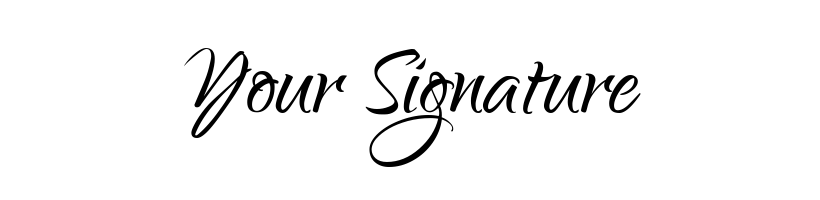
\includegraphics[width=0.12\textwidth]{figures/signature.png}
\end{figure}
% {\raggedright L. C. Strang}
\begin{flushright}
Your Name Here
\end{flushright}

% \hspace{10cm}\hrulefill

This thesis is an original work by the author reporting research done alone or in collaboration with other authors. 
This section provides a chapter-by-chapter summary of the author's contributions and the publication status of all material.

\begin{description}
  \item[Chapter 1] is a comprehensive literature review written by the author for this thesis.
    It is an original work of the author.
    This chapter has not and will not be submitted for publication.
  \item[Chapter 2] is...
\end{description}

%%% Local Variables: 
%%% mode: latex
%%% TeX-master: "../thesis.tex"
%%% End: 
A long list of acknowledgements, inside jokes, etc




% include each chapter...
%\setcounter{chapter}{-1}  % start chapter numbering at 0
\graphicspath{{Figures/Introduction}}

\chapter{Introduction}\label{ch:intro}

\section{Background and motivation}\label{intro:sec:background}
% Purpose of this literature review 
This literature review provides a summary on drug resistance in \textit{Mycobacterium tuberculosis} (MTB), focusing on identifying drug resistance-conferring mutations. This review examines mutations conferring resistance, methods for detecting drug resistance, and innovations in these methods. As for scope, this review covers genomic studies using Next-Generation Sequencing (NGS).

Tuberculosis (TB) is an infectious disease primarily affecting the respiratory system  with symptoms including cough with bloody mucus, fever, and fatigue \cite{pai2016}. TB is caused by infection with species in the \mtb-complex (MTBC), a group of closely related bacteria. MTBC includes MTB, the pathogen responsible for human TB, and additional species that infect humans and other animals \cite{gagneux2018}. Generally, MTB is used synonymously with MTBC \cite{riojas2018} due to high genetic similarity among MTBC strains \cite{gagneux2018}. Therefore, this review will refer to the causative agent of TB as \textit{Mycobacterium tuberculosis} or MTB.

TB impacts global significantly with $\sim$ 10 million people being diagnosed in 2022, and is the second leading causes of death (second to COVID-19) with $\sim$ 1.3 million deaths \cite{who2022}. Drug resistance (DR) worsens global anti-TB challenges, as DR renders standard treatments less effective, leading to higher mortality rates and treatment costs \cite{who2022}. Therefore, global and national health programs need to be vigilant with detecting drug resistance in order to inform effective treatment strategies, ultimately mitigating the burden of TB.
\subsection{The Treatment of Tuberculosis and the Critical Role of Detecting Drug Resistance}

Effective treatment against TB is crucial in global efforts, as cases remain high \cite{who2022}. Historically, standard drug treatments have been successful, however, as Multi-Drug resistant TB (MDR-TB) and Extensively Drug Resistant TB (XDR-TB) emerged, they complicated treatment regimens \cite{whitney2016}.  MDR- and XDR-TB demand treatments that more complex, prolonged, and resource-intensive, burdening both patient and provider \cite{whitney2016}. 

\subsubsection{Treatment Regimens for Drug-Susceptible Tuberculosis}
Drug-Susceptible TB (DS-TB) remains the most common form of the disease \cite{who2022}, with well-established treatment regimens \cite{whitney2016}. The standard treatment for DS-TB consists of first-line drugs, and given proper adherence, can effectively resolve TB cases. In addition to TB resolution, appropriate prescription and adherence to DS-TB protocols can prevent drug resistance \cite{whitney2016,islam2017drug,khawbung2021, pai2016}. 

DS-TB treatment lasts about 6 months and involves two phases: an induction phase and a consolidation phase. The induction phase lasts for two months with the following prescribed antibiotics: rifampicin (also called rifampin), isoniazid, pyrazinamide, and ethambutol \cite{horsburgh2015}. The consolidation phase lasts 4 months, where the patient is prescribed rifampicin and isoniazid. In addition, treatments can extend to 9 months if tests still indicate infection after the standard 6-month treatment. Alternatively, shorter treatmets have been developed, where in 2022, the World Health Organisation (WHO) approved a shorter 4-month regimen. This shorter regimen includes 2 months of isoniazid, rifapentine, moxifloxacin , and pyrazinamide, followed by 2 months of rifapentine, moxifloxacin, and pyrazinamide \cite{queensland_health_2023}

Despite the high efficacy of DS-TB treatments, drug-resistance still poses a significant threat to global TB control. Compared to DS-TB, treatments for MDR- and XDR-TB are intricate, costly and drawn-out.

\subsubsection{Treatment Regimens for Drug-Resistant Tuberculosis}
When designing Drug-Resistant TB (DR-TB) treatments, health programs need to introduce an alternative set of drugs.  These drugs are designated as second-line and include new and repurposed compounds \cite{Heyckendorf2018}. Treatments including them are expensive and induces adverse side-effects, making them taxing on the patient, healthcare provider and the national healthcare systems\cite{whitney2016}. 

Drug resistance refers to the ability of MTB to tolerate effects of anti-TB drugs, rendering standard treatments as ineffective \cite{who2022}. Drug resistanceid  classified as: multi-drug-resistant TB (MDR-TB), pre-extensively drug-resistant TB (pre-XDR-TB) and extensively drug-resistant TB (XDR-TB) \cite{Heyckendorf2018,Viney2100361}. MDR-TB is resistant to rifampicin and isoniazid and pre-XDR-TB fulfills the MDR-TB requirements, but is resistant to any fluoroquinolone (FQ).  Lastly, XDR-TB fulfills pre-XDR-TB requirements, but is resistant to any second-line injectable drug (SLID) \cite{Heyckendorf2018,Viney2100361}.

Additional drugs are used to treat MDR-TB, and the WHO categorises them into three groups. Group A includes fluoroquinolones, namely levofloxacin and moxifloxacin, as well as new and repurposed drugs such as bedaquiline and linezolid \cite{Aguilar2023, whoguide2022}. Group B includes newer drugs such as cycloserine and terizidone, and repurposed drugs such as clofazimine. Lastly, Group C includes amikacin/streptomycin (SLIDs), ethambutol, delamanid, pyrazinamide, imipenem-cilastatin/meropenem, ethionamide/prothionamide, and p-aminosalicylic acid \cite{whoguide2022}. These drugs are critical as they form the defense against MDR-TB. 

As recommended by the WHO, treatment for MDR-TB lasts for 18 months, where the WHO recommends a combination of Group A and Group B drugs, with Group C agents used if needed \cite{whoguide2022}. These drugs can impair kidney function, induce liver damage, and trigger cognitive impairments \cite{sturdy2011mdr}. The side effects can call for a different combination of drugs \cite{whitney2016}, further lengthening treatment. 

If a patient harbors an XDR-TB strain, then a more individualised treatment approach that is dependent on the drug susceptibility status of the isolate. The healthcare provider would have develop a treatment regimen from Group A, B and C drugs which lasts for 18 months or longer \cite{who2022,whoguide2022}. 

To tackle the issues of treatment duration and side effects, the WHO has suggested shorter regimens for MDR-TB \cite{whoguide2022}. These treatments are under conditional recommendation, as more clinical trials are conducted\cite{whoguide2022}. The WHO recommends a 6-month regimen for MDT-TB and Pre-XDR-TB, abbreviated as BPaLM (bedaquiline, pretomanid, linezolid 600 mg, moxifloxacin).

Furthermore, a 9-month all-oral regimen has been developed by the WHO and is appropriate for patients with MDR-TB with no observed evidence of FQ resistance. This treatments includes bedaquiline, administered for 6 months, with a blend of FQs (levofloxacin and moxifloxacin), ethionamide, ethambutol, a high dose of isoniazid, pyrazinamide and clofazimine for 4 months. After this 4-month period, if sputum tests are positive, clofazimine should be introduced and the additional blend may be extended to 6 months. Ultimately, the final 5 months will consist of the FQs, clofazimine, ethambutol and pyrazinamide. If ethionamide contraindication is present, e.g. in preganant patients, linezolid (600mg) can be introduced daily for 2 months \cite{whoguide2022}. This all-oral treatment has the added benefit of lowering infection risk and venous thrombosis that occurs during intravenous administration of drugs which require a central long line \cite{whitney2016}. Overall, these newer treatments aim to reduce the adverse side effects of second-line drugs and the burden on the healthcare system.

In conclusion, treatments for both DS-TB and MDR-, Pre-XDR-, and XDR-TB have show success, despite the rising prevalence of drug-resistant cases. However, as treatment regimens become more complex for drug-resistant cases, timely identification of drug resistance is crucial to ensure effective treatment. 

\subsection{Drug Susceptibility Testing for Tuberculosis}
Timely knowledge of drug resistance is essential as it prevents ineffective treatment and inhibits the proliferation of drug-resistant populations in the patient, preventing the patient's condition from worsening. \cite{whitney2016}. Healthcare providers identify the presence of drug-resistance through the process of drug susceptibility testing (DST). DST involves isolating and culturing the patient's samples (usually sputum) and conducting tests to determine which anti-TB agents the sample is resistant or susceptible to. These tests can return a categorical result in the form of a binary, \enquote{resistant} or \enquote{susceptible}, or the result can be numerical in the form of minimum inhibitory concentration (MIC) \cite{whitney2016, islam2017drug}. 

Currently there are three modalities of DST: Phenotypic DST (pDST), Genotypic DST (gDST) and Whole Genome Sequencing DST (WGS-DST) \cite{who2022}. At a surface-level, pDST measures the growth (or lack thereof) of the bacterium in the presence of anti-TB drugs. This is usually a lengthy process, as MTB is slow growing bacilli \cite{gagneux2018}, and is prone to false positives for certain drugs \cite{Yusoof2022}. Therefore, gDST provides much faster and accurate testing by looks for well-known drug-resistance conferring mutations to particular drugs. This process provides a significant cut in DST duration, as it only needs 2 hours to complete.
Despite rapid testing, gDST still suffers from false results as it only screens for well-known resistance markers \cite{whitney2016}. Overcoming this limitation, WGS-DST sequences and evaluates the entire genome to find mutations that confer drug resistance \cite{whitney2016}. This section will discuss the methodology of these 3 DST modalities and their strengths and weaknesses.

\subsubsection{Phenotypic Drug Susceptibility Testing (pDST)}
pDST is the process where drug resistance is indicated by the phenotype of the MTB isolate. If the proportion of growth in the presence of an anti-TB drug exceeds the established critical concentration - the specific concentration of drug where a susceptible MTB isolate's growth would be inhibited - then the isolate is deemed resistant \cite{who2022, who2021tb}. 

There are two ways of conducting pDST: on solid media and liquid media. Solid medium pDST involves growth media such as Löwenstein-Jensen (LJ) or Middlebrook 7H10/7H11 agar. The proportion of growth in the presence of anti-TB drugs suggests resistance, and the turnaround time for results is about 28–42 days \cite{who2022}. Alternatively, liquid medium pDST uses systens such as the Mycobacterial Growth Indicator Tube (MGIT) containing Middlebrook 7H9 liquid media. Systems such as MGIT, rely on proxy measures like fluorescence or chemical changes to ascertain growth and resistance in the presence of anti-TB drugs\cite{Yusoof2022}. Liquid media pDST is than solid media, taking about 14 days, however it is not without it's limitations. pDST is reliable and recommended for first-line drugs, and certain second-line injectables and fluoroquinolones. But MGIT shows high false positive rates for pyrazinamide, demanding specialised lab staff to supervise testing \cite{who2018tb}. 

Although pDST is recommended by the WHO in some cases \cite{whoguide2022}, several limitations prevent its ubiquitous use. The turnaround time is lengthy, delaying critical treatment decisions, and false positives can lead to unnecessary use of expensive second-line drugs, extending treatment and increasing the risk of adverse side effects. Additionally, conducting pDST requires appropriate lab infrastructure and skilled technicians, which is a hurdle in countries with economic challenges, especially since these countries often bear the greatest burden of MTB infections \cite{who_world_bank_2022}.

\subsubsection{Genotypic Drug Susceptibility Testing}

Genotypic Drug Susceptibility Testing (gDST) involves detecting a pre-determined set of resistance-conferring mutations in the MTB isolate. The mutations primarily occur in genes that encode for the targets of anti-TB drugs. For example, to detect resistance to rifampicin, gDST methods focus on identifying mutations in the \textit{rpoB} gene. A common resistance-conferring mutation is S531L, which indicates resistance against rifampicin \cite{sinha2020detection}. 

Tools for gDST include Nucleic Acid Amplification Tests (NAATs) and, less commonly, Line Probe Assays (LPAs). Examples of NAATs include the Xpert MTB/RIF test, which detects both the presence of MTB and rifampicin resistance in about two hours \cite{iram2015rapid}. This is significantly faster than pDST, allowing it to be used in clinical settings, with the major infrastructure needs being constant power supply and provider training \cite{whitney2016}. However, the main issue with gDST is its limited mutation coverage. Tests like Xpert MTB/RIF and LPAs target specific mutations known to confer resistance, potentially missing rare or novel mutations. This can result in false negatives, where gDST fails to detect a resistance-conferring mutation \cite{Yusoof2022}. For example, Xpert MTB/RIF screens for mutations in the rifampicin resistance-determining region (RRDR) -  an 81-bp regions of the \textit{rpoB} gene - where more than 95\% of rifampicin resistance-conferring mutations are detected \cite{rahman2016comparison,musser1995antimicrobial}, this excludes the remainder of the \textit{rpoB} gene.  I491F mutation in the \textit{rpoB} gene associated with drug resistance but is not included in the RRDR \cite{mon2022first}, therefore Xpert MTB/RIF would overlook this mutation, resulting a false negative. To mitigate this, the WHO recommends pDST to be used complementarily to finalise drug susceptibility results \cite{Yusoof2022, whoguide2022}. But the issue with pDST confirmation is that it extends the time required for diagnosis, possibly counteracting the speed advantage of gDST.

\subsubsection{Whole-Genome Sequencing in Drug Susceptibility Testing (WGS-DST)}

WGS-DST overcomes the issue of limited scope and low sensitivity with gDST and the extensive time and resource requirments of pDST, allowing for a comprehensive look into the MTB genome. WGS leverages NGS technologies to sequence the MTB genome entirely and then search for mutations that are associated with drug resistance. Generally,  Illumina WGS experienced more frequent utilisation due to it's higher per-base accuracy \cite{marin2022benchmarking}, however with improvements to long-read sequencing, Nanopore by Oxford Nanopore Technologies (ONT) \cite{hall2023evaluation, smith2020assessing} and PacBio \cite{meehan2018} are becoming more prevalent.

For WGS-DST to occur, patient samples must first be cultured. Following this, library preparation can take place and sequencing can be initiated. Once the isolates have been sequenced, their reads can be mapped to a reference genome,  and for MTB it is the H37Rv reference genome \cite{meehan2018}. Once aligned, the reads will then flow through a variant calling pipeline, to identify genetic variants within the isolate. The specific pipeline is yet to be standardised, and it is a pressing issue as different pipelines can yield different results \cite{walter2020genvar,meehan2018}. 

After completing the WGS sequencing, read mapping and variant calling, a list of variants are produced. With this list and a catalogue containing known mutations associated with drug resistance, the clinician can determine the drug resistance profile of the isolate. This is done by cross-referencing mutations from the variant list with the mutation catalogue. 

In 2021, the WHO published a catalogue including resistant-conferring mutations to 13 anti-TB drugs. This catalogue included a list of MTB mutations that are associated with drug resistance with high confidence, and were developed from using over 40,000 isolates from 46 countries. A lower number of mutations were identified for new and repurposed drugs such as bedaquilline \cite{Walker2022}. This catalogue was updated in 2023 to include data from a larger dataset of isolates and updates mutations for new and repurposed drugs \cite{WHOcatalog}, resulting in the catalogue including mutations for all anti-TB drugs endorsed by the WHO. Ultimately, the WHO catalog is a standardised reference document which lists and describes the confidence of mutations associated with drug resistace and their selection critera \cite{Walker2022,WHOcatalog}. This catalogue also served national TB programs and diagnostic assay manufacturers to develop more accurate DST tools \cite{WHOcatalog}. The scope of the WHO catalogue was deliberately made to be non-exhaustive, as recommendations were only made for mutations with high confidence \cite{Walker2022}.

The main benefits offered by WGS DST is it's ability to comprehensively test for resistance in a wide array of drugs, including variants that are missed by commercial gDST assays \cite{dean202225}. The time needed for WGS-DST ranges from 1 -2 weeks \cite{whitney2016}, being significantly faster than pDST. However, this is slower than the $\sim$ 2 hour turnaround for gDST assays. But, with the cultures available, the sequencing workflow can be optimised to 3-5 days\cite{whitney2016}. Access to WGS technologies is being improved by the development of portable sequencing technologies such MinION developed by ONT, allowing direct testing on sputum samples \cite{hall2023evaluation,smith2020assessing}. 

With the adoption of WGS-DST increasing, widespread implementation is limited by technological and infrastructure needs in low-income regions. Additionally, standardisation in bioinformatic analysis pipelines is highly needed to ensure consistency in DST results across different settings \cite{meehan2018, world2018use, inzaule2021genomic}. 

While, WGS-DST offers a broad window to find novel resistance conferring mutations, it is still affected by incomplete coverage. The process of masking, where sections of the genome are excluded from analysis results in blindspots that are not accounted for when investigating for mutations \cite{modlin2021exact}. This remains a key region for investigation. 

Overall, WGS offers deep and almost exhaustive insight into possible mutations that may cause drug-resistance in Mtb - making it a highly promising modality for widespread DST usage \cite{whitney2016}. This can be improved through innovation in better filters and analysis of previously excluded genomic regions. 
 \subsection{Investigating Mutations in Masked Genomic Regions}
 
\subsubsection{Masking Practices in Mtb Genomic Analysis}

During genomic analysis of the Mtb genome, about 10\% of the Mtb genome commonly needs to be masked \cite{meehan2018}, in a conservative attempt to lower the prevalence of erroneous variant calls. These incorrect calls are a technological limitation of using short-read genome mapping. Short reads (100 - 250bp), are difficult to align to genomic regions that are repetitive or contain homologous sequences \cite{li2008mapping, li2014toward}.  Therefore, the variant caller may identify incorrect mutations, or miss mutations altogether \cite{marin2022benchmarking}. 

These masked regions contain repetitive and homologous sequences, consisting mostly of the \textit{pe/ppe} gene family \cite{marin2022benchmarking}. This gene family, comprised of 168 genes, adopt versatile roles in MTB virulence \cite{gagneux2018,d2023pe}.  As drug-resistant mutation catalogues exclude the masked regions \cite{Walker2022}, investigation into the \textit{pe/ppe} gene family for drug-resistance conferring mutations needs to be conducted. 

\subsubsection{The \textit{pe/ppe} Gene Family and Drug Resistance}

The \ppe gene family proteins contain a conserved \textit{pe} (Proline-Glutamic Acid) or \textit{ppe} (Proline-Proline-Glutamic Acid) motif in their N-terminal domain, with their C-terminal domains being variable, both in sequence and length \cite{d2023pe, cole1998deciphering}. This gene family is over-represented in pathogenic mycobacteria \cite{d2023pe, gagneux2018} and is diverse in function, likely being an adaptation to host's immune system \cite{de2019immune}. 

The \ppe gene family's distribution within the genome is optimised for targeted gene control. Although, the distribution appears as random, the \textit{pe/ppe} genes are packaged into operons consisting of a \textit{pe} gene proceeded by a \textit{ppe} gene \cite{d2023pe, tundup2006clusters}. 

The \textit{pe/ppe} gene family can be characterised their variable C-terminal domains. The PE family can be classified into the PE sub-family and the PE-Polymorphic GC-rich (PE-PGRS) sub-family \cite{cole1998deciphering,gey2006evolution}.  The PE-PGRS sub-family has high GC-content (approximately 80\%), and are highly variable and prone to recombination \cite{gey2006evolution, daleke2012general}. The PPE family can also be classified into two subfamilies, namely the PPE and PPE-Major Polymorphic Tandem Repeat (PPE-MPTR) \cite{cole1998deciphering,gey2006evolution}. The PPE-MPTR sub-family proteins have been observed to be exceptionally large, with secreted proteins exceeding 3000 amino acids in length \cite{hermans1992characterization,cole1998deciphering, gey2006evolution}. 

The \ppe gene family are also involved in antibiotic resistance \cite{d2023pe}. Mutations within \ppe regions have are associated with drug resistance, specifically through the action of gene-pair mutations. A pair of genes, consisting of a gene encoding a drug target and a \ppe gene are associated in a drug-resistant isolate \cite{d2023pe}. Examples include \textit{KatG-PPE54}, where mutations in both \textit{KatG}, whose gene product activates isoniazid \cite{islam2017drug} and \textit{PPE54} were observed in isoniazid resistant isolates. Likewise, another gene pair was \textit{rpoB} (encodes drug target for rifampicin \cite{islam2017drug}) and \textit{PPE-54} were observed in a rifampicin-resistant isolate. Other gene pairs were observed for common anti-TB drugs such as ethambutol and streptomycin \cite{cui2016bioinformatics}. Therefore genes in the \ppe gene family are prime targets for investigation. 

Aside from gene-pair interactions, mutations in certain sub-families have been shown to be enriched in resistant isolates. Specifically, numerous members of the PE-PGRS sub-family were observed in XDR-TB isolates \cite{kanji2015characterization}.  Moreover, mutations in PPE genes were  associated with an expansion in Isoniazid resistance \cite{hang2019whole}.

Additionally, \ppe proteins alter MTB cell functioning, rendering them resistant to anti-TB drugs. For example, PE11, a protein with esterase activity is involved with cell wall remodelling, increasing the hydrophobicity of the cell surface and its impermeability to anti-TB drugs \cite{singh2016pe11}.

Currently, genes in the \ppe family are commonly masked in standard analyses, meaning potential drug resistance-conferring mutations may be overlooked, motivating changes to standard masking practices. This will accommodate the discovery of newer mutations, thus improving mutation catalogue accuracy. 

\subsection{Re-evaluating the Masking Approach}

Masking involves excluding regions of the MTB genome, as they are comprised of repetitive, highly homologous and GC-rich regions, rendering them difficult to analyse (Figure 2). These regions can lead to fluctuations in coverage due to reads mapping to multiple locations which may misinterpreted as deletions. 

Masked regions of the genome contain the \ppe gene family, sequences homologous to other regions of the genome and mobile genetic elements \cite{meehan2018,marin2022benchmarking,modlin2021exact}. As a result, their exclusion comes at a cost of missed alignments, causing potentially missed drug-resistance conferring mutations. Specifically the exclusion of the \ppe gene family is costly, due to mutations in those regions, as mentioned previously, have been associated with drug-resistance \cite{cui2016bioinformatics, kanji2015characterization} and they are integral to MTB virulence \cite{d2023pe}.  Therefore, this motivates the need for more accurate and concentrated masking practices. 

\begin{figure}[H]
    \centering
    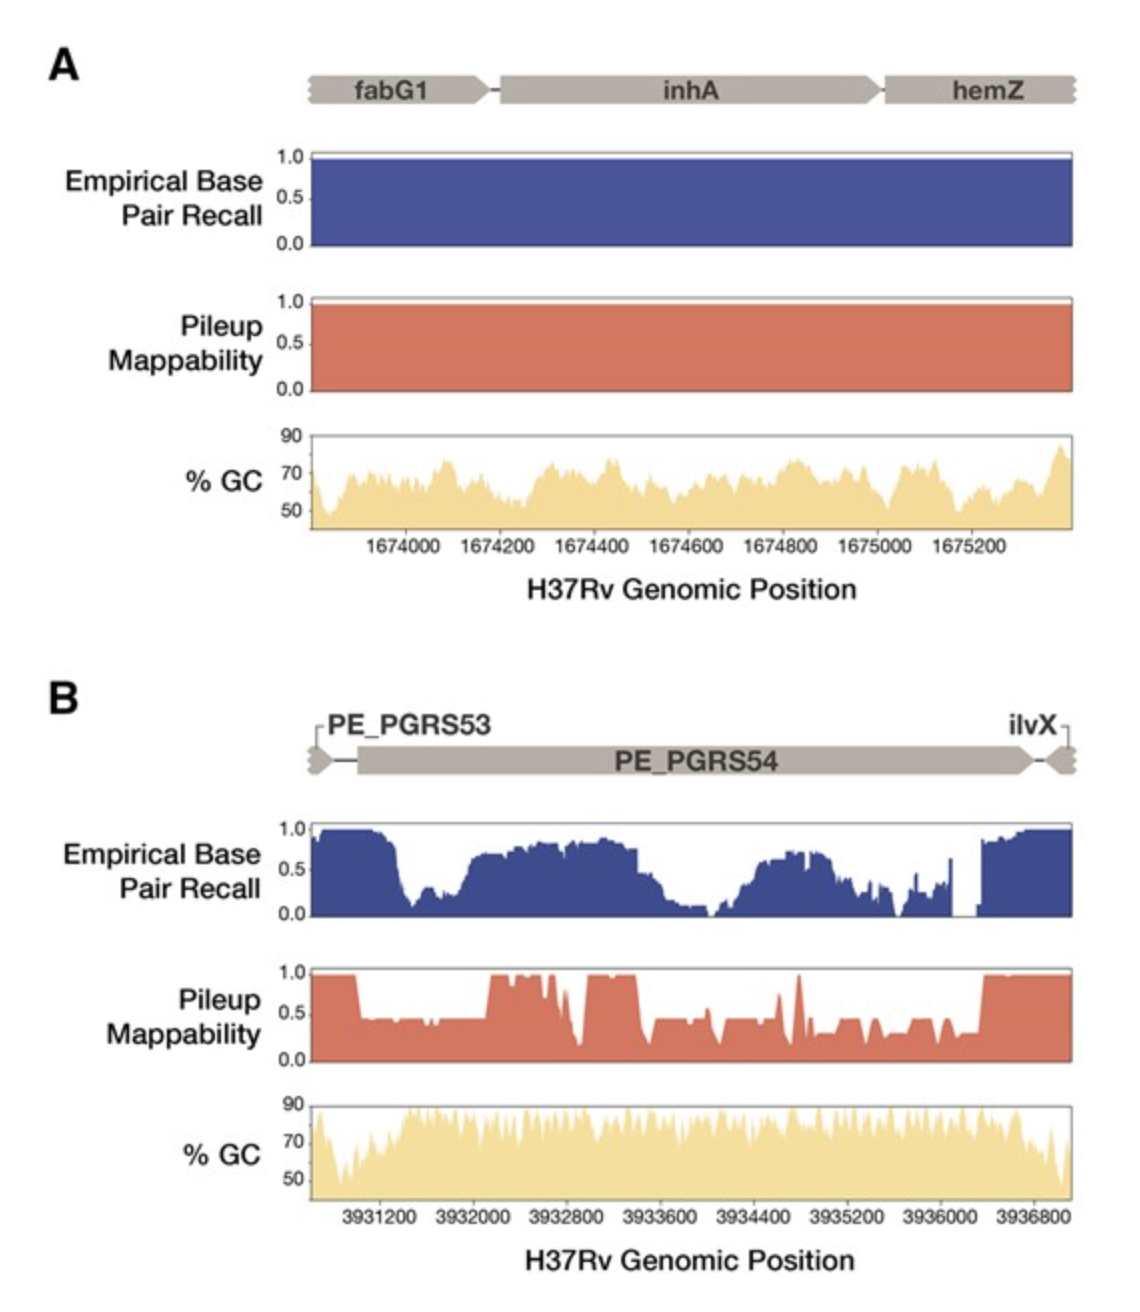
\includegraphics[width=0.7\linewidth]{figures/Screen Shot 2024-11-01 at 5.22.47 am.png}
  \caption{Comparison of empirical base pair recall (EBR), pileup mappability, and GC content across selected regions of the H37Rv MTB genome. (A) Shows the region including \textit{fabG1}, \textit{inhA}, and \textit{hemZ}, which has high EBR and mappability. (B) Shows a region containing \textit{PE\_PGRS53} and \textit{PE\_PGRS54}, illustrating the lower empirical recall and mappability (Marin \etal, 2022).}
\end{figure}

Empirical studies investigating the efficacy of conservative masks has supported the need for newer masking regimes. A benchmarking study by Marin \etal, found that approximately 90\% of all false positive variant calls occurred in only a 65kb sliver of the MTB genome when no masking is applied \cite{marin2022benchmarking}. This represents about 1.5\% of the MTB genome, and comparing that to the 10\% traditionally masked highlights the unnecessary exclusion of highly mappable regions. Reinforcing this, Modlin et al., found that low-coverage regions, or  \enquote{blind spots} were less prevalent in previously masked regions, while paradoxically, many of these blind spots were identified in regions that had been included in analyses \cite{modlin2021exact}. These studies also discovered that the \ppe gene family could be analysed with the use of newer masks. Marin et al., reported that 52/168 or about one-third of \ppe genes had high mappability, although the sub-families PE-PGRS and PPE-MPTR showed lower mappability \cite{marin2022benchmarking}. Moreover, Modlin \etal reported the distribution of blind spots were lower than expected in \ppe regions and that certain \ppe genes do not have any blind spots \cite{modlin2021exact}. 

\begin{figure}[H]
    \centering
    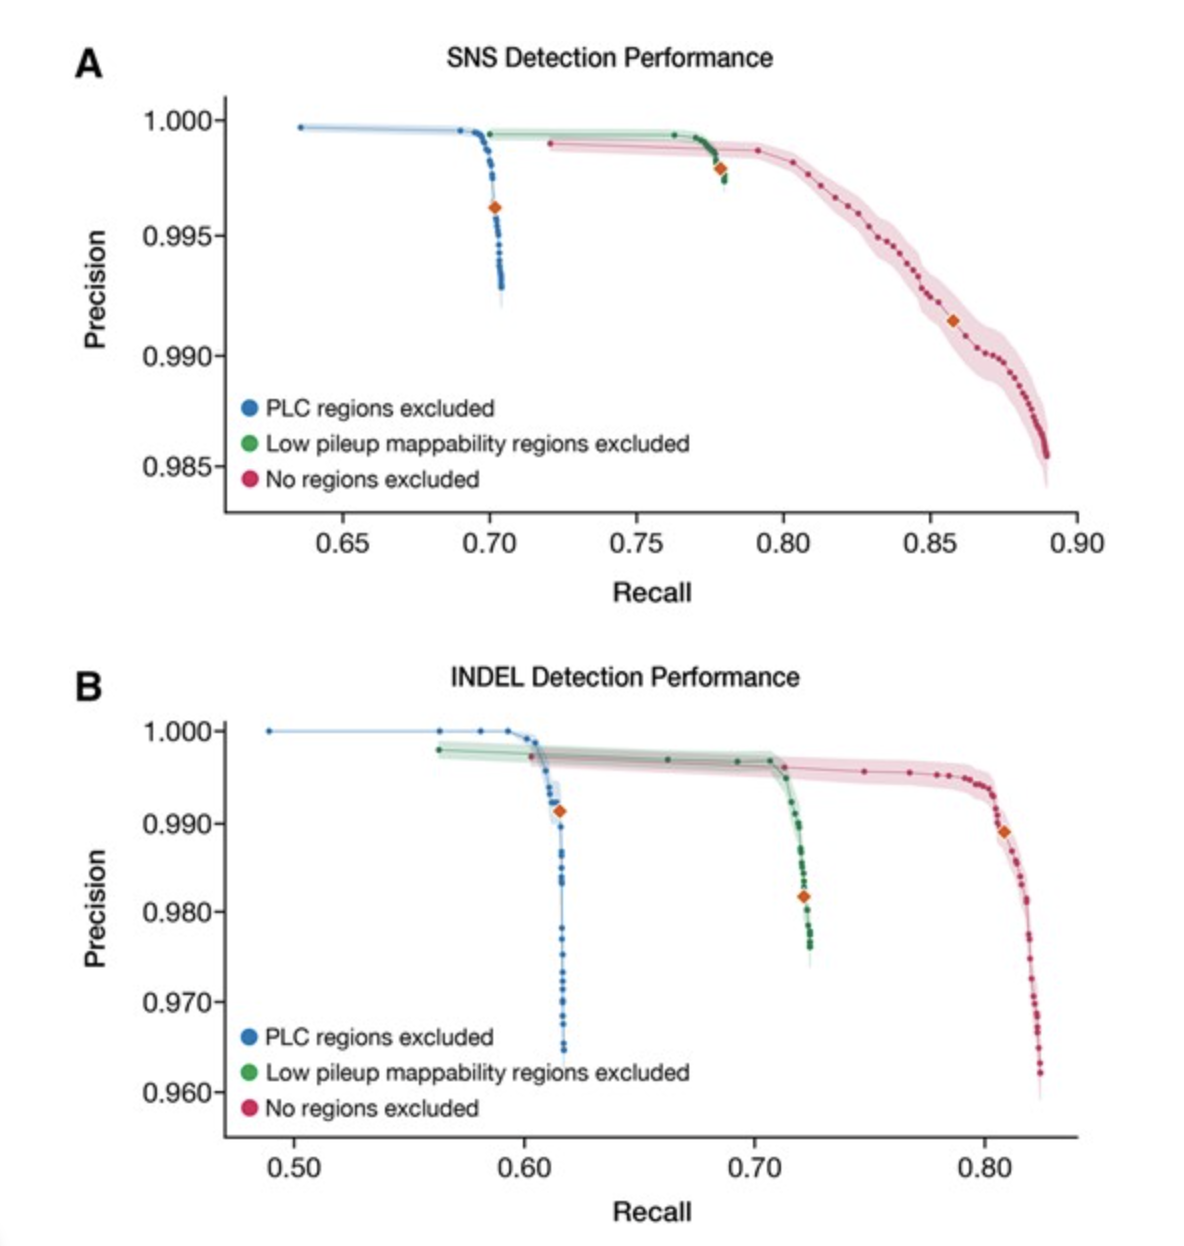
\includegraphics[width=0.7\linewidth]{figures/Screen Shot 2024-11-01 at 5.26.51 am.png}
    \caption{Mean single nucleotide substitution (SNS) and INDEL variant calling approaches across different masks. (A) SNS detection performance was assesed with three masking strategies: permissive masks (low pileup mappability regions excluded), no masking (no regions excluded) and traditional masks (PLC regions excluded). (B) Short INDEL performance was also included. The orange diamonds represent mean precision and recall at MQ threshold of 40. (Marin \etal, 2022) }
\end{figure}

Establishing the importance of revised masking practices and the need to analyse \ppe genes, newer masking protocols have been developed. Firstly, Marin \etal intended to refine currently excluded regions, labelling them as \enquote{Refined Low-Confidence} (RLC) regions. RLC regions span only about 4$\%$ of the genome, in contrast to the 10$\%$ that are usually masked. This mask was developed through optimisation of certain metrics used in variant calling. Marin \etal focused on Mapping Quality (MQ), which measure the probability that a read was incorrectly aligned to the reference genome. By optimising the threshold for MQ, Marin \etal, were able to significantly reduce the size of the excluded regions whilst maintaing precision without sacrificing recall (Figure 3) \cite{marin2022benchmarking}. In addition, Modlin \etal had bench-marked different sequencing workflows used by Illumina WGS, and analysed the distribution of blind-spots across the genome. As a result providing more accurate masks \cite{modlin2021exact}. 

Accurate masking enables detailed insight into previously masked genomic regions, especially the regions accomodating the \ppe gene family. This will facilitate thorough investigation in regions previously ignored for resistance-conferring mutations. These mutations may potentially explain drug-resistant phenotypes that do not have an associated mutation, or it may predict drug resistance in other cases. Thus, prospective genotype-phenotype associations developed from applying newer masks can provide meaningful contributions to mutation catalogues, ultimately enhancing drug-resistance detection and treatment of drug-resistant tuberculosis.  

\section{Research objectives}\label{intro:sec:objectives}

\section{Contributions}\label{intro:sec:contributions}

\section{Thesis structure}\label{intro:sec:structure}

% !TeX root = ../main.tex
\graphicspath{{Figures/Methods}}

\chapter{Methods}\label{ch:methods}

\section{Data acquisition and catalogue formation}\label{methods:sec:data_agg}
This chapter comprehensively details the computational and statistical methods that were developed to produce an end-to-end machine learning pipeline for predicting drug resistance for M.tb and flaggin candidate variants to explain False Negative samples. Constructing a robust dataset for model-training and candidate variant identification, approximately $45,000$ M.tb genomes were downloaded from the Sequence Read Archives (SRA) and European Nucleotide Archive (ENA) repositories \cite{sra_infra_2022, ena_infra_2024}.

The methods is partitoned into $3$ phases. Firstly, an initial mapping is constructed using the WHO mutation catalogue \cite{WHOcatalog} and correspondingly updated with updated ``expert-rule'' heuristics. Secondly, a variant-discovering pipeline utilised identified FN samples to aggregate uncatalogued, highly significant variants. Thirdly, these variant features were supplied to a parallelised, single-layer neural network, designed to map sparse variant inputs directly to continuous, multi-drug probability outputs.

The remaining sections of this chapter follow the structure: Section 2.1 outlines data ingestion from the WHO-catalogue, Section 2.2 details rule-based variant filtering to updte the WHO-catalogue; and Section 2.3 defines the neural network parameters, custom loss functions, and post-training ablation study. 

\subsection{The WHO catalogue of mutations}
To construct features representing resistance-conferring variants from the WHO-catalogue of mutations, variant-feature mapping was done. The WHO catalogue MS Excel files were retrieved from the "mutation-catalogue-2023" repository \cite{WHOcatalog}. The variant features were constructed by forming a string of the variant position, reference allele and alternate allele(s): \texttt{POS\_REF\_ALT}. With the selected variants being restricted to ``Associated with Resistance'' or ``Associated with Resistance-interim'', the final confidence grade for each variant was limited to 1 or 2. A final confidence variant of $3$ meant ``Not Associated with Resistance'', and a grade of $4$ and $5$ meant ``Not Associated with Resistance-interim'' and ``Not Associated with Resistance'', respectively \cite{Walker2022, WHOcatalog} (Figure~\ref{fig:who}). Using these constraints, the catalogue was constructed into a map of 15 anti-TB drugs with their corresponding resistance-conferring variants.\\

\begin{figure}[H]
  \centering
   \begin{tabular}{|c|c|}
    \hline
    Group & Classification \\
    \arrayrulecolor{red}\hline
    1 & Assoc R \\
    \arrayrulecolor{red}\hline
    2 & Assoc w R-interim \\
    \arrayrulecolor{red}\hline
    3 & Uncertain significance \\
    \arrayrulecolor{black}\hline
    4 & Not assoc with R-interim \\
    \hline
    5 & Not assoc with R \\
    \hline
  \end{tabular}
  \\[1cm]
  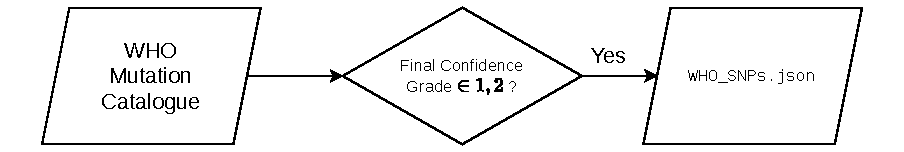
\includegraphics[width=\textwidth]{figures/who_snps.pdf}
  \caption{WHO SNP filtering process}
  \label{fig:who}
\end{figure}

\subsection{Updating the WHO catalogue with expert rules}
To update the WHO catalogue with ``expert rules'' released in the latest version \cite{WHOcatalog}, rule-based variant-filtering and variant-feature mapping was employed.

The WHO expert rules were acquired from the WHO-catalogue report released in 2023 \cite{WHOcatalog}. The expert-rules were implemented to extract variants from $\sim$45,000 M.tb VCF files. The M.tb VCF files were produced primarily from an alternative pipeline with variant-calling being done with Snippy \cite{tseemann_snippy} and variant annotation by SnpEff \cite{cingolani2012program}. The M.tb genomes were downloaded from the Sequence Read Archive (SRA) and ENA genome databases \cite{sra_infra_2022, ena_infra_2024}.

The expert rules that could be incorporated into the pipeline were rules 6–11, as the older rules involved processing MIC data or phenotypic measurements which were out of the scope for our project. Rule 6 stated any non-synonymous variant in the Rifampicin Resistance Determining Region (RRDR) of \textit{rpoB} (codons 426–452) were upgraded to final confidence grade (group) 2, meeting our criteria and thus, collected. Rule 7 collected variants for Fluoroquinolone (FQ) cross-resistance, any \textit{gyrA/gyrB} variant graded 1 or 2 for Levofloxacin (LFX) but 3 for Moxifloxacin (MFX), was upgraded to group 2 and vice versa. Rule 8 collected variants for Isoniazid-Ethionamide (INH-ETO) cross-resistance, where any \textit{inhA/fabG1} variant graded for INH but 3 for ETO cases was upgraded to 2 for the ETO and vice versa. Rule 9 collected variants for Bedaquiline-Clofazimine (BDQ-CFZ) cross-resistance, with any \textit{Rv0678/mmpL5} variants graded 1 or 2 for BDQ but group 3 for CFZ were upgraded to level 2 for CFZ. Rule 10 concerned pooling Loss-of-Function (LoF) variants in \textit{ddn, fbiA, fbiB, fbiC, fgd1, Rv2983} for Delamanid and Pretomanid DLM/PA. Rule 11 more broadly collected non-synonymous variants including LoF, earlyy stop, frameshift, gene deletion, or start-loss, in \textit{ethA, gid, katG, pncA, Rv0678, rpsA, ddn, fbiA, fbiB, fbiC, fgd1, Rv2983, tlyA}, were upgraded to group 2 for their respective drugs. Lastly from the previous version of expert-tules\cite{miotto2018}, any pncA variant was assumed to be resistant,  and correspondingly upgraded to group 1 or 2. Additionally, variants were harvested from intergenic regions aswell, with only synonymous variants  being skipped. Using the said expert rules, additional variants were harvested from $\sim$45,000 VCF files. Lastly, they were incorporated into the relevant drug index from WHO mapping.

\begin{figure}[htbp]
  \centering
  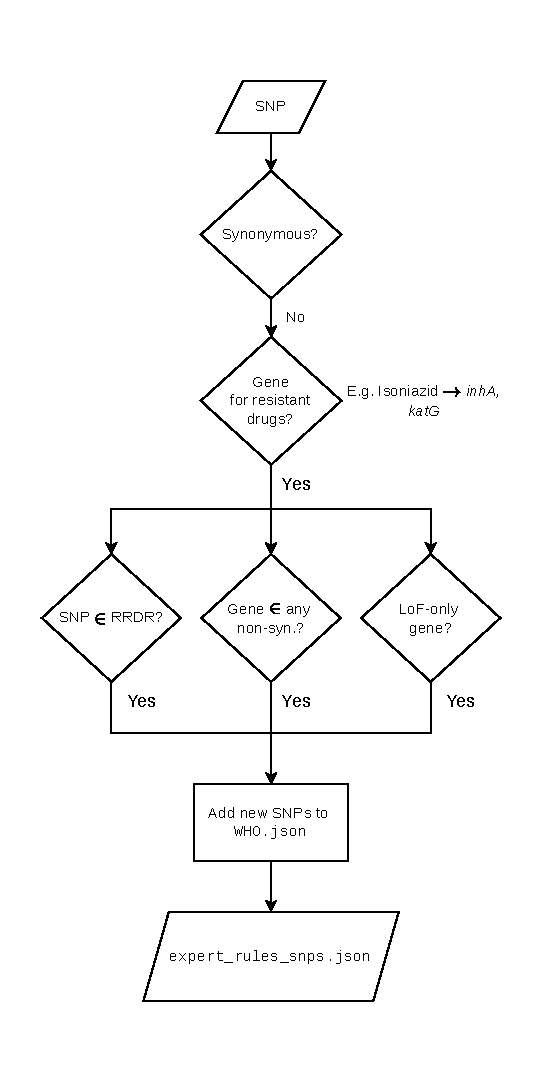
\includegraphics[width=1\textwidth]{figures/er.drawio-1.pdf}
  \caption{Expert rules SNP filtering process}
  \label{fig:er}
\end{figure}

\section{Augmenting updated catalogues}

\subsection{Resistance profiling and identification of False Negatives}
To identify False Negative (FN) samples for 22 anti-TB drugs, TB-Profiler (v6.6.6) \cite{phelan2019integrating} was use employed to profile over 45,000 M.tb genomes. 45,000 M.tb genomes were retrieved from the SRA and ENA databases \cite{sra_infra_2022, ena_infra_2024}. Of the 45,840 genomes retrieved, 45,702 were sequenced using short-read Illumina sequencing \cite{Bentley2008} and 138 were sequenced using Oxford Nanopore sequencing \cite{Jain2018}. Profiling for each sample was done with \texttt{tb-profiler predict} with parameters \texttt{--txt --no\_trim}. The mutation database used by TB-Profiler was version 2 of the WHO catalogue \texttt{WHO-v2-Strict} \cite{phelan2019integrating}. 

Resistance profiles produced from TB-Profiler were compared to phenotypic susceptibility data for at least 1 drug per sample. The confusion matrix was defined as follows:
\begin{itemize}
  \item \textbf{True Positive:} Both resistance-prediction and phenotype was Resistant.
  \item \textbf{False Negative:} The resistance-prediction was Susceptible, whereas the phenotype was Resistant. These files were our primary focus.
\item \textbf{True Negative:} Both resistance-prediction and phenotype were Susceptible.
\item \textbf{False Positive:} The resistance-prediction was Resistant, whereas the phenotype was Susceptible.
\end{itemize}

Using these classifications, we isolated samples that were FN for a particular drug (Figure~\ref{fig:filt}). 

\subsection{Identifying resistance-conferring candidate variants}
To augment the updated WHO catalogue map, for all variants identified in the FN samples, a Fishcer's Exact test was conducted. For 22 anti-TB agents, a $|\text{M.tb genomes}| \times |\text{Unique variants}|$, binary variant matrix was constructed. Using TN samples as a control, $p$-values (p-vals) and Odd Ratios (ORs) were calculated using the Fischer's Exact Test. To identify variants that were significant in the FN samples and associated with resistance, a filter of $-log_{10}(pval) \leq 5$ and $-log_{10}(OR) \> 1$ was imposed. Any p-value or OR that had a calculated value of \texttt{inf} or \texttt{-inf} were ignored.

To ensure the significant variants were not markers of M.tb lineage \cite{gagneux2018}, a variant was removed if it was in a list of identified lineage markers \cite{freschi2021population}. Lastly, if the variant was not already included in the updated WHO map, then the variant was added for that specific drug (Figure~\ref{fig:filt}) 


\begin{figure}[htbp]
  \centering
  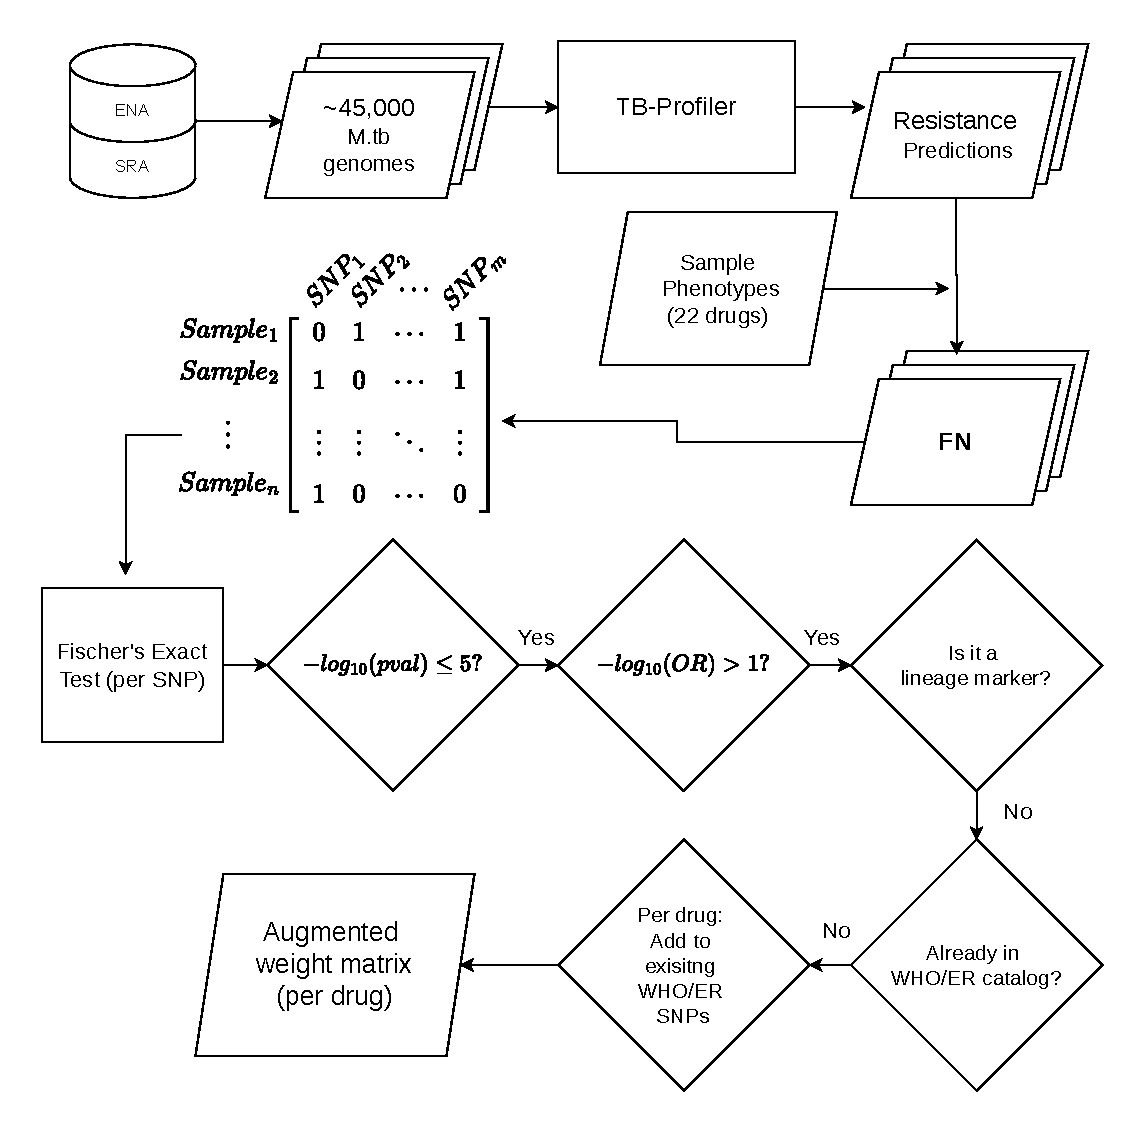
\includegraphics[width=1\textwidth]{figures/filt.drawio.pdf}
  \caption{Filtering SNP from FNs and augmented existing catalogues}
  \label{fig:filt}
\end{figure}

\section{Probabilistic implementation of a resistance prediction tool}

This section outlines the implementation and training framework of the parallelised, neural network built to provide a transition from rigid, static catalogue look-ups to a dynamic probabilistic method. Simulatenously, probabilities for 15 anti-TB drugs would be predicted. As shown in Figure~\ref{fig:train} the network adjusts weights based off a Loss function, which in this case was a customised Binary Cross-Entropy (BCE) A mask was implemented to ignore phenotypic data that was missing, ensuring proper training of the network. Following training, a threshold sweep was conducted to find prediction thresholds that maximised sensitivity, with a specificity constraint. Finally, an ablation study was conducted to quantify the impact of variants harvested from FNs had on the sensitivity.

This section is outlined as follows: Section 2.3.1 defined the layer connectivity matrices, weight scaling factors, and anchor regulariser equations; Section 2.3.2 describes data splitting criteria, strategies to address class imbalances, and a masked approach to gradient updates. Lastly, Section 2.3.3 estbalishes the threshold evlauation sweeps and feature ablation criteria.

\subsection{Network architecture and weights initisiatilisation}
To produce a resistance prediction for a sample, for a particular drug, a probability was produced a neuron with a sigmoid activation function. Firstly, the variant from a sample VCF was transformed into a binary input tensor $\mathbf{x} \in \{0,1\}^{26k\times1}$. If the sample contained a variant in the WHO map (with $\sim26k$ variants), then it was encoded by 1, 0, if not. The input tensor, $\mathbf{x}$ was passed into neuron that represents a particular drug. The weights for the neuron was set by the $n$ variants included for the drug in the WHO variant map. Those $n$ variants had an edge weight of 1 and the remaining $\sim26k-n $ variants were set to 0. Before training, the bias for the network was set to 0. Ultimately, the summation of inputs and weights $\mathbf{w}^{T}\mathbf{x}$,were passed into the sigmoid activation function, $$\sigma = \frac{1}{1+e^{-x}}$$ which produced a probability, $\hat{p} \in [0,1]$. A threshold of $\hat{p} > 0.5$ was applied for a resistance prediction (Figure~\ref{fig:onescheme}). 

\begin{figure}[htbp]
  \centering
  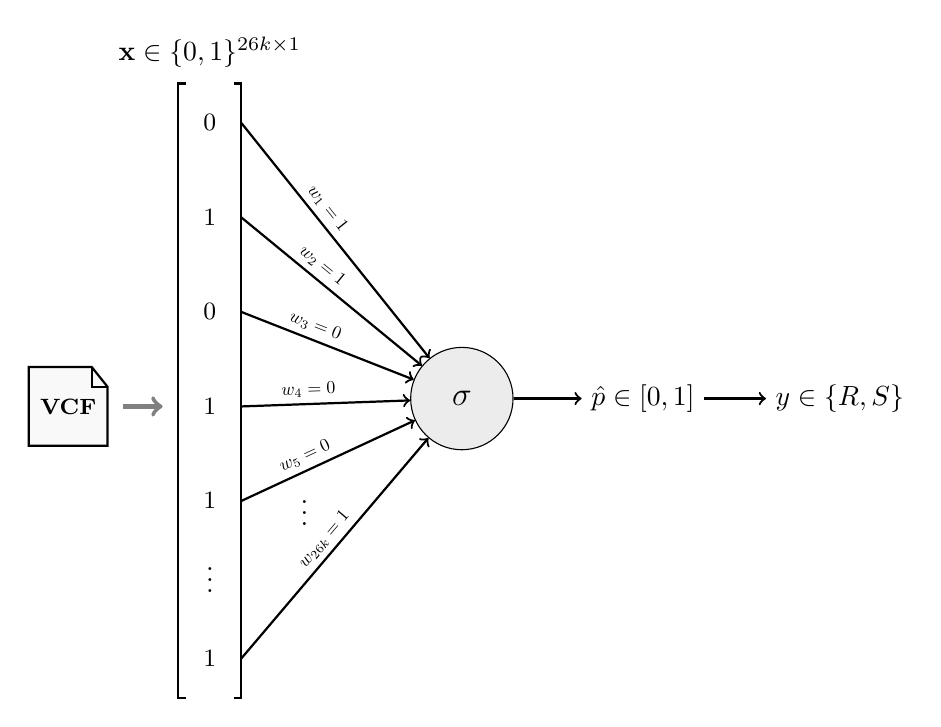
\begin{tikzpicture}[
      % Style for the binary digits inside the input vector
      input_node/.style={draw=none, minimum size=0.6cm, font=\small},
      % Style for the single MUCH LARGER Sigmoid processing node
      sigm_node/.style={circle, draw=black, minimum size=1.3cm, fill=gray!15, font=\large\bfseries},
      % Style for plain text/labels
      plain/.style={draw=none}
  ]

      % --- 0. VCF FILE ICON ---
      \draw[thick, fill=gray!5] (-2.3, 0.4) -- (-1.5, 0.4) -- (-1.3, 0.15) -- (-1.3, -0.6) -- (-2.3, -0.6) -- cycle;
      \draw[thick] (-1.5, 0.4) -- (-1.5, 0.15) -- (-1.3, 0.15);
      \node[font=\footnotesize\bfseries] at (-1.8, -0.1) {VCF};
      
      % Arrow from VCF file to Input Vector
      \draw[->, ultra thick, gray] (-1.1, -0.1) -- (-0.6, -0.1);


      % --- 1. INPUT LAYER (26k SNP Binary Vector) ---
      \draw[thick] (-0.3, 4.0) -- (-0.4, 4.0) -- (-0.4, -3.8) -- (-0.3, -3.8); 
      \draw[thick] (0.3, 4.0) -- (0.4, 4.0) -- (0.4, -3.8) -- (0.3, -3.8); 
      
      \node[plain] at (0, 4.4) {$\mathbf{x} \in \{0,1\}^{26k \times 1}$};

      % Binary Elements
      \node[input_node] (in1) at (0, 3.5)  {$0$};
      \node[input_node] (in2) at (0, 2.3)  {$1$};
      \node[input_node] (in3) at (0, 1.1)  {$0$};
      \node[input_node] (in4) at (0, -0.1) {$1$};
      \node[input_node] (in5) at (0, -1.3) {$1$};
      \node[plain]      (indot) at (0, -2.2) {$\vdots$};
      \node[input_node] (in26k) at (0, -3.3) {$1$};


      % --- 2. THE LARGE SIGMOID NEURON (Centered at Y=0) ---
      \node[sigm_node] (sig1) at (3.2, 0) {$\sigma$};


      % --- 3. SYNAPSE CONNECTIONS ---
      % All inputs converge cleanly into the large single neuron node
      \draw[->, thick] (0.4,3.5) -- node[above, pos=0.4, scale=0.65, sloped, black] {$w_1=1$} (sig1);
      \draw[->, thick] (0.4, 2.3) -- node[above, pos=0.4, scale=0.65, sloped, black] {$w_2=1$} (sig1);
      \draw[->, thick] (0.4, 1.1) -- node[above, pos=0.4, scale=0.65, sloped, black] {$w_3=0$} (sig1);
      \draw[->, thick] (0.4,-0.1) -- node[above, pos=0.4, scale=0.65, sloped, black] {$w_4=0$} (sig1);
      \draw[->, thick] (0.4, -1.3) -- node[above, pos=0.4, scale=0.65, sloped, black] {$w_5=0$} (sig1);
      \node[plain] (dot) at (1.2,-1.35) {$\vdots$};
      \draw[->, thick] (0.4, -3.3) -- node[above, pos=0.5, scale=0.65, sloped, black] {$w_{26k}=1$} (sig1);



      % --- 4. INTERMEDIATE LAYER (Scalar Probability Output) ---
      \node[plain] (p1) at (5.5, 0) {$\hat{p} \in [0,1]$};
      \draw[->, thick] (sig1) -- (p1);

      % --- 6. OUTPUT LAYER (Final Single Drug Susceptibility Class) ---
      \node[plain] (y1) at (8, 0) {$y \in \{R, S\}$};
      \draw[->, thick] (p1) -- (y1);

  \end{tikzpicture}
  \caption{Schematic for one neuron with weights specified for a particular drug}
  \label{fig:onescheme}
\end{figure}

For all 15 anti-TB drugs from the WHO catalogue, 15 neurons corresponding to each drug produced an output vector $\mathbf{y}\in {R,S}^{15\times1}$ (Figure~\ref{fig:fullschem}).

\begin{figure}
  \centering
  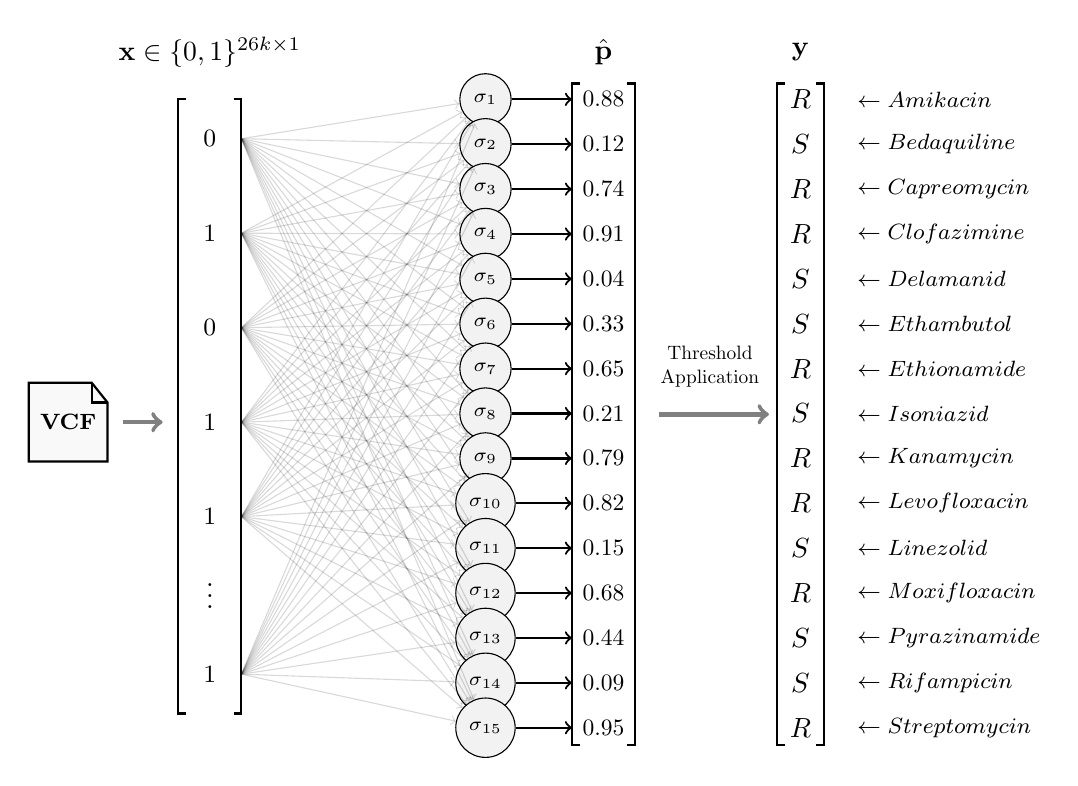
\begin{tikzpicture}[
      % Style for the binary digits inside the input vector
      input_node/.style={draw=none, minimum size=0.6cm, font=\small},
      % Style for the 15 Sigmoid processing nodes
      sigm_node/.style={circle, draw=black, minimum size=0.65cm, fill=gray!10, font=\scriptsize},
      % Style for plain text/labels
      plain/.style={draw=none},
      % Custom style to draw a document/file icon
      file_icon/.style={
          draw, thick, fill=white,
          append after command={
              % Draws the folded corner of the paper icon
              [shift={(-0.15,-0.2)}] (\numexpr\tikzlastnode\relax.north east) -- 
              ++(-0.25,0) -- ++(0,0.25) -- cycle
          }
      }
  ]

      % --- 0. VCF FILE ICON (Shifted right from -3.3 to -1.8) ---
      \draw[thick, fill=gray!5] (-2.3, 0.4) -- (-1.5, 0.4) -- (-1.3, 0.15) -- (-1.3, -0.6) -- (-2.3, -0.6) -- cycle;
      \draw[thick] (-1.5, 0.4) -- (-1.5, 0.15) -- (-1.3, 0.15);
      \node[font=\footnotesize\bfseries] at (-1.8, -0.1) {VCF};
      
      % Shorter Arrow from VCF file to Input Vector
      \draw[->, ultra thick, gray] (-1.1, -0.1) -- (-0.6, -0.1);


      % --- 1. INPUT LAYER (26k SNP Binary Vector) ---
      % Vector Brackets
      \draw[thick] (-0.3, 4.0) -- (-0.4, 4.0) -- (-0.4, -3.8) -- (-0.3, -3.8); 
      \draw[thick] (0.3, 4.0) -- (0.4, 4.0) -- (0.4, -3.8) -- (0.3, -3.8); 
      
      \node[plain] at (0, 4.6) {$\mathbf{x} \in \{0,1\}^{26k \times 1}$};

      % Binary Elements
      \node[input_node] (in1) at (0, 3.5)  {$0$};
      \node[input_node] (in2) at (0, 2.3)  {$1$};
      \node[input_node] (in3) at (0, 1.1)  {$0$};
      \node[input_node] (in4) at (0, -0.1) {$1$};
      \node[input_node] (in5) at (0, -1.3) {$1$};
      \node[plain]      (indot) at (0, -2.2) {$\vdots$};
      \node[input_node] (in26k) at (0, -3.3) {$1$};


      % --- 2. 15 SIGMOID NODES LAYER ---
      \foreach \j in {1,...,15} {
          \pgfmathsetmacro{\ypos}{4.0 - (\j-1) * 0.57}
          \node[sigm_node] (sig\j) at (3.5, \ypos) {$\sigma_{\j}$};
      }


      % --- 3. DENSE SYNAPSE CONNECTIONS ---
      \foreach \j in {1,...,15} {
          \draw[->, thin, opacity=0.15] (0.4,3.5) -- (sig\j);
          \draw[->, thin, opacity=0.15] (0.4, 2.3) -- (sig\j);
          \draw[->, thin, opacity=0.15] (0.4, 1.1) -- (sig\j);
          \draw[->, thin, opacity=0.15] (0.4, -0.1) -- (sig\j);
          \draw[->, thin, opacity=0.15] (0.4, -1.3) -- (sig\j);
          \draw[->, thin, opacity=0.15] (0.4, -3.3) -- (sig\j);
      }


      % --- 4. INTERMEDIATE LAYER (Probability Vector shifted left to X=5.0) ---
      \foreach \j / \prob in {
          1/0.88, 2/0.12, 3/0.74, 4/0.91, 5/0.04, 
          6/0.33, 7/0.65, 8/0.21, 9/0.79, 10/0.82, 
          11/0.15, 12/0.68, 13/0.44, 14/0.09, 15/0.95
      } {
          \pgfmathsetmacro{\ypos}{4.0 - (\j-1) * 0.57}
          \node[plain] (p\j) at (5.0, \ypos) {\scalebox{0.85}{$\prob$}};
          % Shorter line endpoint target changed to 4.6
          \draw[->, thick] (sig\j) -- (4.6, \ypos);
      }
      
      % Probability Vector Brackets (Shifted to encompass X=5.0)
      \draw[thick] (4.7, 4.2) -- (4.6, 4.2) -- (4.6, -4.2) -- (4.7, -4.2); 
      \draw[thick] (5.3, 4.2) -- (5.4, 4.2) -- (5.4, -4.2) -- (5.3, -4.2); 
      \node[plain] at (5.0, 4.6) {$\hat{\mathbf{p}}$};


      % --- 5. THRESHOLD APPLICATION TRANSITION (Compensated leftward shift) ---
      \draw[->, ultra thick, gray] (5.7, 0) -- node[above, black, align=center, scale=0.7, yshift=10pt, xshift=-2pt] {Threshold\\Application} (7.1, 0);


      % --- 6. OUTPUT LAYER (Final Vector shifted left to X=7.5) ---
      \foreach \j / \res / \drug in {
          1/R/Amikacin, 2/S/Bedaquiline, 3/R/Capreomycin, 4/R/Clofazimine, 
          5/S/Delamanid, 6/S/Ethambutol, 7/R/Ethionamide, 8/S/Isoniazid, 
          9/R/Kanamycin, 10/R/Levofloxacin, 11/S/Linezolid, 12/R/Moxifloxacin, 
          13/S/Pyrazinamide, 14/S/Rifampicin, 15/R/Streptomycin
      } {
          \pgfmathsetmacro{\ypos}{4.0 - (\j-1) * 0.57}
          
          % Final categorical value
          \node[plain] (y\j) at (7.5, \ypos) {$\text{\res}$};
          
          % Right Annotation (Drug Names shifted closer)
          \node[plain, anchor=west, font=\footnotesize] at (8.1, \ypos) {$\leftarrow \text{\drug}$};
      }

      % Final Classification Vector Brackets (Shifted to encompass X=7.5)
      \draw[thick] (7.3, 4.2) -- (7.2, 4.2) -- (7.2, -4.2) -- (7.3, -4.2); 
      \draw[thick] (7.7, 4.2) -- (7.8, 4.2) -- (7.8, -4.2) -- (7.7, -4.2); 

      \node[plain] at (7.5, 4.6) {$\mathbf{y}$};

  \end{tikzpicture}
  \caption{Neural Net schematic for 15 drugs}
  \label{fig:fullschem}
\end{figure}


\subsection{Training regime and optimisation}
To provide an alternative to rigid look-up mechanics of a catalogue and to capture continuous probabilistic thresholds for multi-drug resistance, a single-layer parallelised neural network was implemented in Tensorflow/Keras. Using this, complex multi-drug weights can be learned from $\sim$45,000 M.tb genomes.

The input layer accepts a high-dimensional, sparse feature tensor $x \in \{0,1\}^{N\times M}$, where $N$ represents the $\sim45,000$ M.tb genomes and $M$ represents the approximately 26,000 distinct variants compiled from the WHO-catalogue. $M > 26,000$ if the expert-rules variants and augmented variants were included. This feature matrix maps directly via a single dense hidden layer to a classification column vector $\hat{p}\in \{0,1\}^{15\times 1}$, where each row stores an independent resistance-prediction across 15 anti-TB drugs. 

The raw linear transformation logits $z$ are evlauated through an element-wise sigmoid activation function: $$ \hat{p}_i = \sigma(z_i) = \frac{1}{1+e^{-z_i}}$$

Rather than implementing a naive weight initisiatilisation strategy, the WHO-catalogue mutation knowledge was transferred. Baseline weight matrices ($W_{init}$) were pre-loaded from the WHO map formation. To optimise training convergence and push the network's boundaries closer to binary classification limits, the kernels scaled by a factor of $10.0$, and all corresponding node biases ($b$) were uniformly preset to a baseline constraint of $-5.0$: $$ W = W_{init}\times 10.0, b_i=-5.0 $$

To ensure the network retains it's biological anchor and avoids extreme weight drift during gradient updates, a custom anchor kernel regulariser was embedded within the loss-layer, penalising squared deviations from the initial configuration using a loss multiplier ($\lambda = 1 \times 10^{-5}$): $$ \Omega(W) = \lambda\sum_{j}(W_j - W_{init,j})^2$$

For efficient network parameter optimisation, while maintaining high predictive stability across highly imbalanced label streams, custom masking was employed. The input matrix, $x$, was split randomly into a $80:20$ train-test split (seeded at \texttt{random\_state=42}). For monitoring training validation and prevent over-fitting, the training set was further split into a manual $80:20$ train-validation configuration. The model was trained over $50$ epochs utilising the AdamW optimiser with a base learning rate ($\alpha$) of $1\times 10^{-3}$, and a batch size of $64$. Training was managed using an automated learning rate decay loop ($\texttt{ReduceLROnPlateau}$, decay factor = $0.2$, patience = $3$ epochs).

Since the phenotypic data for each sample included resistance data for at least one anti-TB drug (out of $22$), many samples had missing values for numerous drugs. Therefore a custom Masked Weigthed Binary Cross-Entropy (BCE) loss function was implemented. This function masked missing phenotypic data ($y_{ij}=\text{NaN}$) during backpropagation to prevent gradients from skewing. In the case of severe class imbalances, where the number of suscptible samples vastly outnumbered resistant samples, positive sample weights were adaptively regularised using the square root of the inverse class ratio calculated from the portion actively being trained: $$ w_{pos,i} = \sqrt{\frac{N_{\text{suscptible},i}}{N_{\text{resistant},i}+10^{-8}}} $$
$$\mathcal{L}_{\text{Masked}} =\frac{\sum_{i=1}^{15} m_i \cdot [w_{\text{pos},i} \cdot y_i log(\hat{p}_i)+(1-y_i)log(1-\hat{p}_i)]}{\sum_{i=1}^15 m_i + 10^{-8}}$$
Where $m_i \in \{0,1\}$ is a binary filter mask, where $m_i=1$ if phenotypic data is present, and $m_i=0$ if absent. 

Following training, the raw prediction vector was processed through a threshold sweep to determine the optimal threshold to predict resitance for that drug. Rather than the inflexible default cutoff ($0.5$), thresholds were dynamically set using receiver operating characteristic (ROC) curves. The threshold that maximised the sensitivity, whilst not degrading the specificity below a pre-defined threshold ($0.80$) were kept. 

Following threshold assignment for each drug, an \textit{in silico} feature ablation assay was conducted. This determined the drop in sensitivity by ablating the specific variant. The variant that were considered for ablation were the significant variants harvested from FN samples, in order to determine the loss of sensitivity caused by their exclusion. Systematically, variant features were excluded by zeroing out their respective index within the input tensor ($W_{\text{ablated}[\text{idx,}d]} = 0.0$). A variant was flagged to cause a significant change in sensitivity if it's exclusion resulted in a sensitivity drop of $\geq 0.05\%$ compared to the unablated baseline sensitivity.

\begin{figure}[htbp]
  \centering
  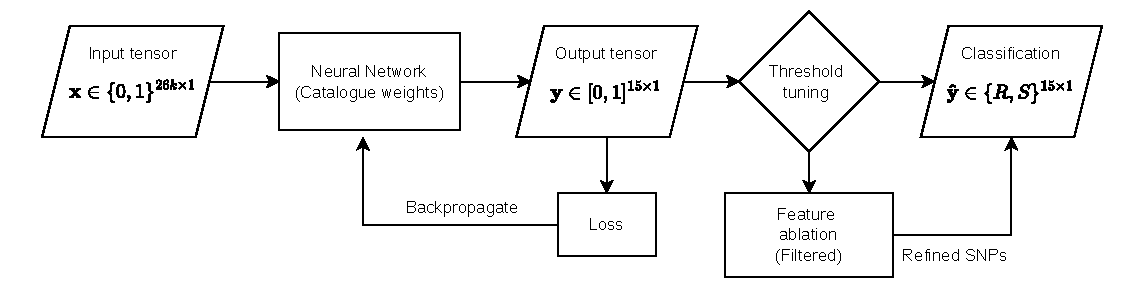
\includegraphics[width=1.2\textwidth]{figures/train.drawio.pdf}
  \caption{Training process}
  \label{fig:train}
\end{figure}

Summarising, the computational and statistical framework in this chapter outlines a pipeline designed to predict the resistance profile for an M.tb sample using an augmented version of the WHO-catalogue. Furthermore, in the process of augmenting the WHO-catalogue using significant variants, candidate variants that can account for the prediction-phenotype discordance in FN samples can be established, given wet-lab validation. The computational performance, validation evlauations, and maps of rescued candidate variants resulting from this pipeline is presented and analysed in Chapter 3.

% !TeX root = ../main.tex
\graphicspath{{Figures/Results}}

\chapter{Results}\label{ch:results}

\section{Classification Performance}\label{results:sec:model_perf}
Following training and post-hoc threshold tuning, model performance was evaluated across 15 anti-TB drugs using sensitivity, specificity and F1 score. Four weight schemes were compared: TB-Profiler (baseline for our model), WHO catalogue (baseline for our weights), WHO updated with expert rules (WHO+ER), and the updated catalogue augmented with filtered variants from FN samples (WHO+ER+Filtered). For each weight scheme, hollow circles denote naiive performance prior to any training or threshold tuning, with only binary weights extracted from the catalogues. Their color-filled circles represent performance post-training and threshold application (Figures~\ref{fig:sens,fig:spec, fig:f1}).

\subsection*{Sensitivity}
Across all 3 weight schemes, sensitivity matched or exceeded TB-Profiler for 13 out of 15 drugs (Figure~\ref{fig:sens}). The untrained baseline anchors highlight sensitivity gains occur post-training and threshold application, rather than catalogue makeup alone, all filled markers sit above their hollow anchors. Under the WHO catalogue baseline, sensitivity increased for all 15 drugs, post-training and threshold tuning. WHO+ER improved for 13 out of 15 drugs, and WHO+ER+Filtered improved for 14 out of 15 drugs. Across most drugs, comparing the three weight schemes, performance was broadly similar. However, there were notable exceptions such as moxifloxacin, where WHO+ER achieved the highest sensitivity among weight schemes. Another drug is delamanid, where both WHO+ER and WHO+ER+Filtered outperformed WHO baseline, suggesting that that catalogue updates with expert rules and FN harvested variants provided meaningful contributions. For bedaquiline, catalogue via expert rules and filtered variants produced the most substantial sensitivity boost out of all drugs, consistent with its newer status in anti-TB treatment.

Clofazimine, delamanid, and linezolid posed a significant challenge to the model, with all weight schemes hitting a ceiling of 0.65 post-training and threshold application. Nevertheless, all WHO weight schemes showed improved performance over TB-Profiler profiler, suggesting the probabilistic framework being able to extract signals even with a smaller set of resistant cases. 

\begin{figure}[H]
  \centering
  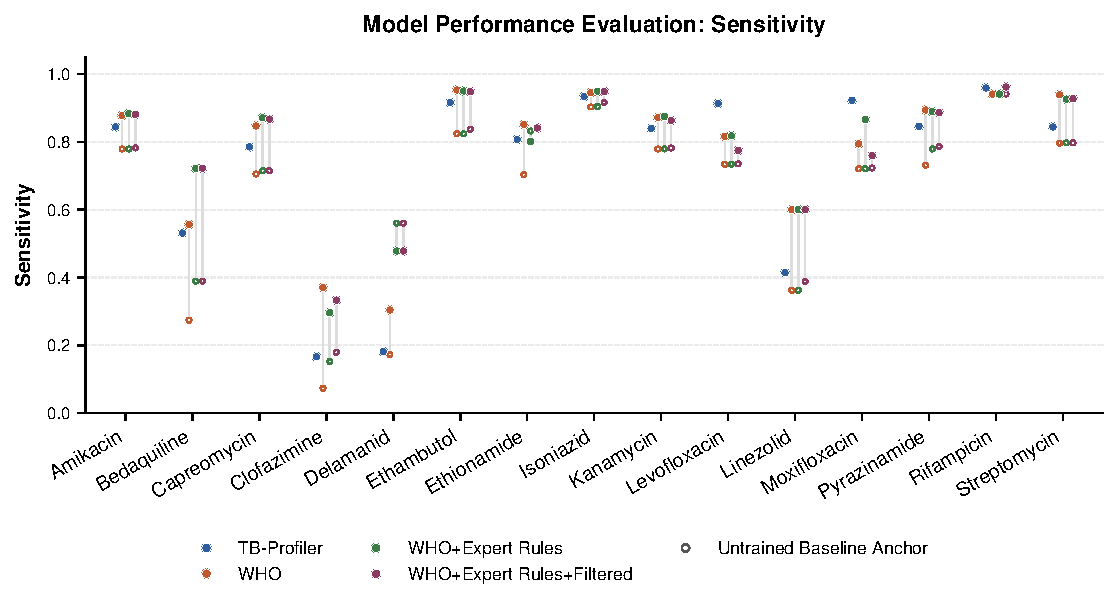
\includegraphics[width=\textwidth]{figures/sensitivity.pdf}
  \caption{Sensitivity of the neural network with tb-profiler as the baseline, WHO, and WHO augmented with
  expert rules, and filtered is shown aswell. The naive pass with only the catalogues encoded as 1s , or 0s
  is shown as empty circles, and the trained model results are filled in.}\label{fig:sens}
\end{figure}

\subsection*{Sensitivity}

As stated in Section 2.5, the threshold tuning procedure enacted a hard specificity boundary of 0.8, and this is visible in Figure~\ref{fig:spec}.
For 8 out of 15 drugs, the learned weights schemes approached or slightly penetrated this floor, illustrating the sensitivity-specificity trade-off accounted for during threshold application. Despite this, ethambutol, clofazimine, delamanid, isoniazid, levofloxacin, moxifloxacin, and ethionamide, specificity for the model weight schemes hovered around TB-Profiler's performance. For rifampicin, the weight schemes matched or even slightly exceeded TB-Profiler's specificity. Subsequently, a specificity difference of $-0.2$ between TB-Profiler and the weight schemes can be observed for amikacin, bedaquiline, capreomycin, kanamycin, pyrazinamide, streptomycin, and linezolid. This gap is a direct manifestation of the specificity trade-off made when boosting sensitivity, ultimately reflecting a higher FP rate, with lowered FN.

\begin{figure}[H]
  \begin{center}
    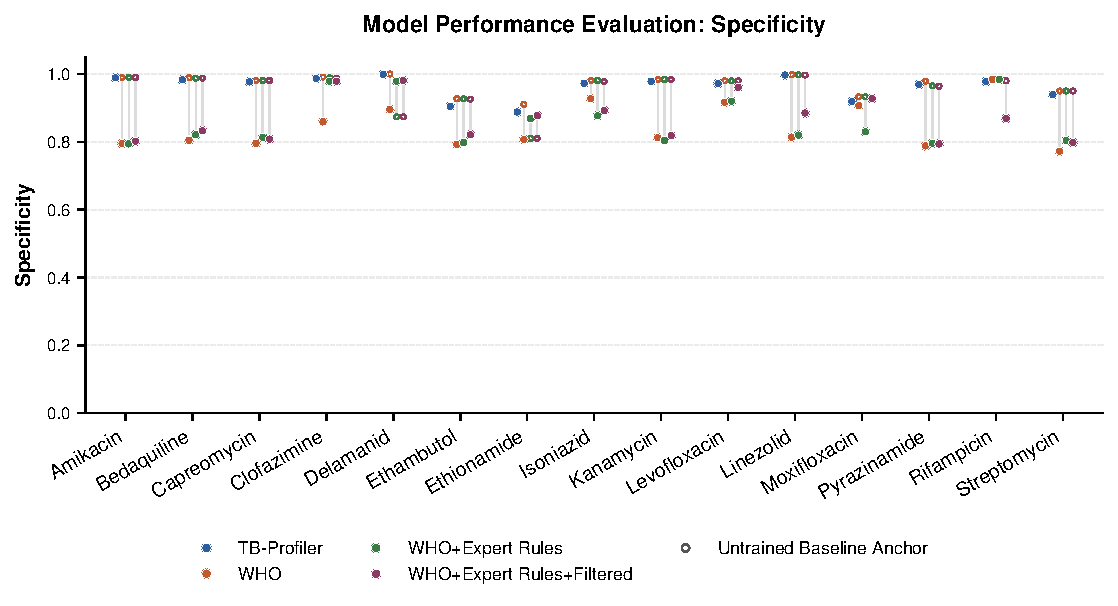
\includegraphics[width=\textwidth]{figures/specificity.pdf}
  \end{center}
  \caption{Specificity of the neural network after training for 15 Anti-TB drugs that had at final confidence
  grading of 1 or 2. TB-profiler (blue) acts as the baseline to show how the neural networks perform with different
  weights. Weights were constructed from the WHO catalogue, and then augmented with expert rules and filtered snps.
  These are represented as hollow circles, and after training, they are represented as filled circles.}\label{fig:spec}
\end{figure}

\subsection*{F1 Score}
The specificity-sensitivity trade-off is reflected in the F1 scores (Figure~\ref{fig:f1}). Drugs where the largest drops in specificity, also showed the largest drops in F1 post-training and threshold tuning: amikacin, bedaquiline, capreomycin, kanamycin, linezolid, and pyrazinamide. This suggests that sensitivity gains were not substantial enough to offset specificity losses under the harmonic mean (F1). The remaining drugs, showed slightly improved or stable F1 compared to TB-Profiler. Clofazimine, delamanid, ethambutol, and rifampicin all showed F1 improvements compared to TB-Profiler. Isoniazid, ethionamide, streptomycin, and moxifloxacin F1 scores remained stable and close to TB-Profiler. Overall, the WHO weight schemes matched or exceeded F1 for 8 out of 15 drugs, demonstrating that specificity costs incurred via threshold tuning does not uniformly degrade overall Classification quality. Lastly, the probabilistic framework provides meaningful gains for drugs where the resistant data is sparse or the WHO catalogue has coverage gaps for. 

\begin{figure}[H]
  \begin{center}
    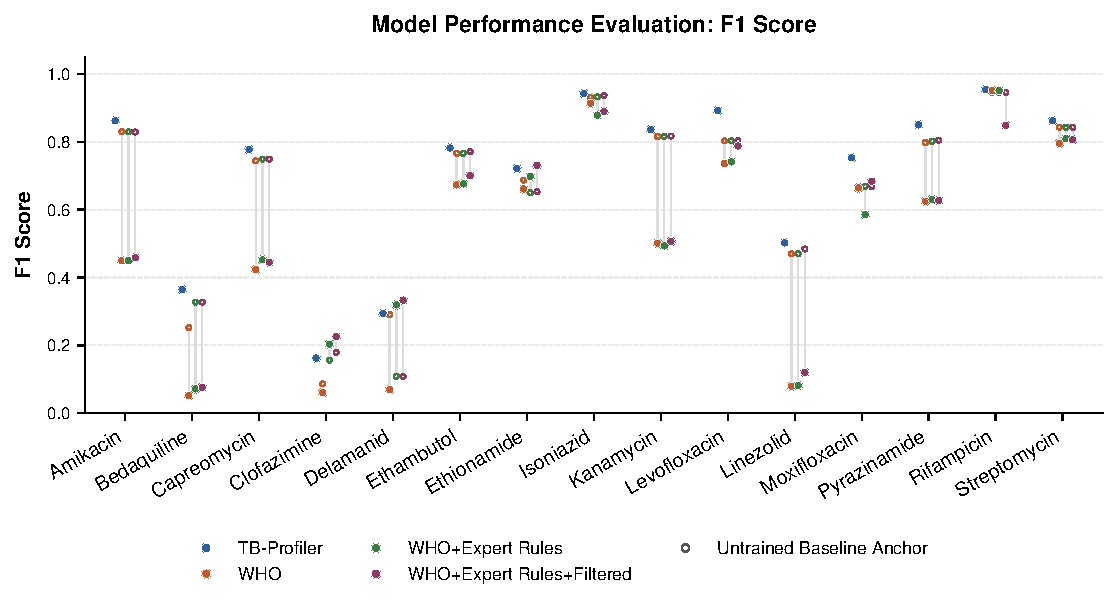
\includegraphics[width=\textwidth]{figures/f1.pdf}
  \end{center}
  \caption{F1 scores of the neural networks, with F1 being the balanced average between specificity and sensitivity.
  In this plot, TB-profiler is used as a baseline, colored in blue, and the untrained networks with shown with hollow
  circles. The trained models are shown with filled circles.}\label{fig:f1}
\end{figure}

\subsection{Training Performance and Convergence}
Training performance was assessed using masked binary cross-entropy loss, AUC, and F1 score over 50 epochs for all weight schemes, here we discuss the WHO+ER+Filtered weight scheme performance (Figure~\ref{fig:filerlr}). Learning curves for other weight schemes and their respective per-drug learning curves can be found in Appendix C. 

Training loss decreased rapidly over the first 20 epochs, falling from approximately 0.500 to near 0.340, before stabilising over the remaining 30 epochs at approximately 0.325. Validation loss followed a close, parallel trajectory, beginning at 0.475, and plateauing around 0.350 with a final test loss of 0.348. Proximity of train, validation, and test loss (within 0.025 of each other) indicates the model generalises well to unseen data without overfitting. Rapid initial descent and stable plateauing over the final 30 epochs are consistent with the expected catalogue weighted scheme performance: the model starts from a biologically grounded position, and requires relatively smaller gradient updates to reach a local minimum. 

Validation AUC climbed from 0.930 at epoch 1 to 0.947 at epoch 50, with training AUC moving from 0.915 to 0.955 over the same interval. Test AUC of 0.9465 falls within training-validation envelope and confirms AUC gains during training reflects effective learning rather than overfitting to training data. Similar to the loss curve, the majority of AUC occurred in the first 20 epochs, following stabilisation. This supports the model reaching its representational capacity early, given the catalogue prior. 

F1 score replicated the same pattern of immediate ascent followed by plateau, with training F1 jumping from $\sim$8.40 to 0.860 and validation F1 from $\sim$0.842 to $\sim$0.857 over 50 epochs, yielding a test F1 of 0.8541. The modest improvement in F1, $\sim$0.060 over 50 epochs, can be understood via the catalogue-weighted models. Catalogue-initialised weights encodes a strong prior, so baseline F1 is expected to be significantly higher than random weights. Training, via gradient-based weight refinement, increments F1 scores which is reflected in the train-validation gap of $\sim$0.003 at convergence. When collated, the loss, AUC, and F1 trajectories indicate an effective training regime with rapid convergence, stable generalisation, and absence of overfitting. The properties are mostly to attribute the biological grounding provided by catalogue weight initialisation and anchor regulariser constraining weight drift during training. 

\begin{figure}[H]
  \begin{center}
    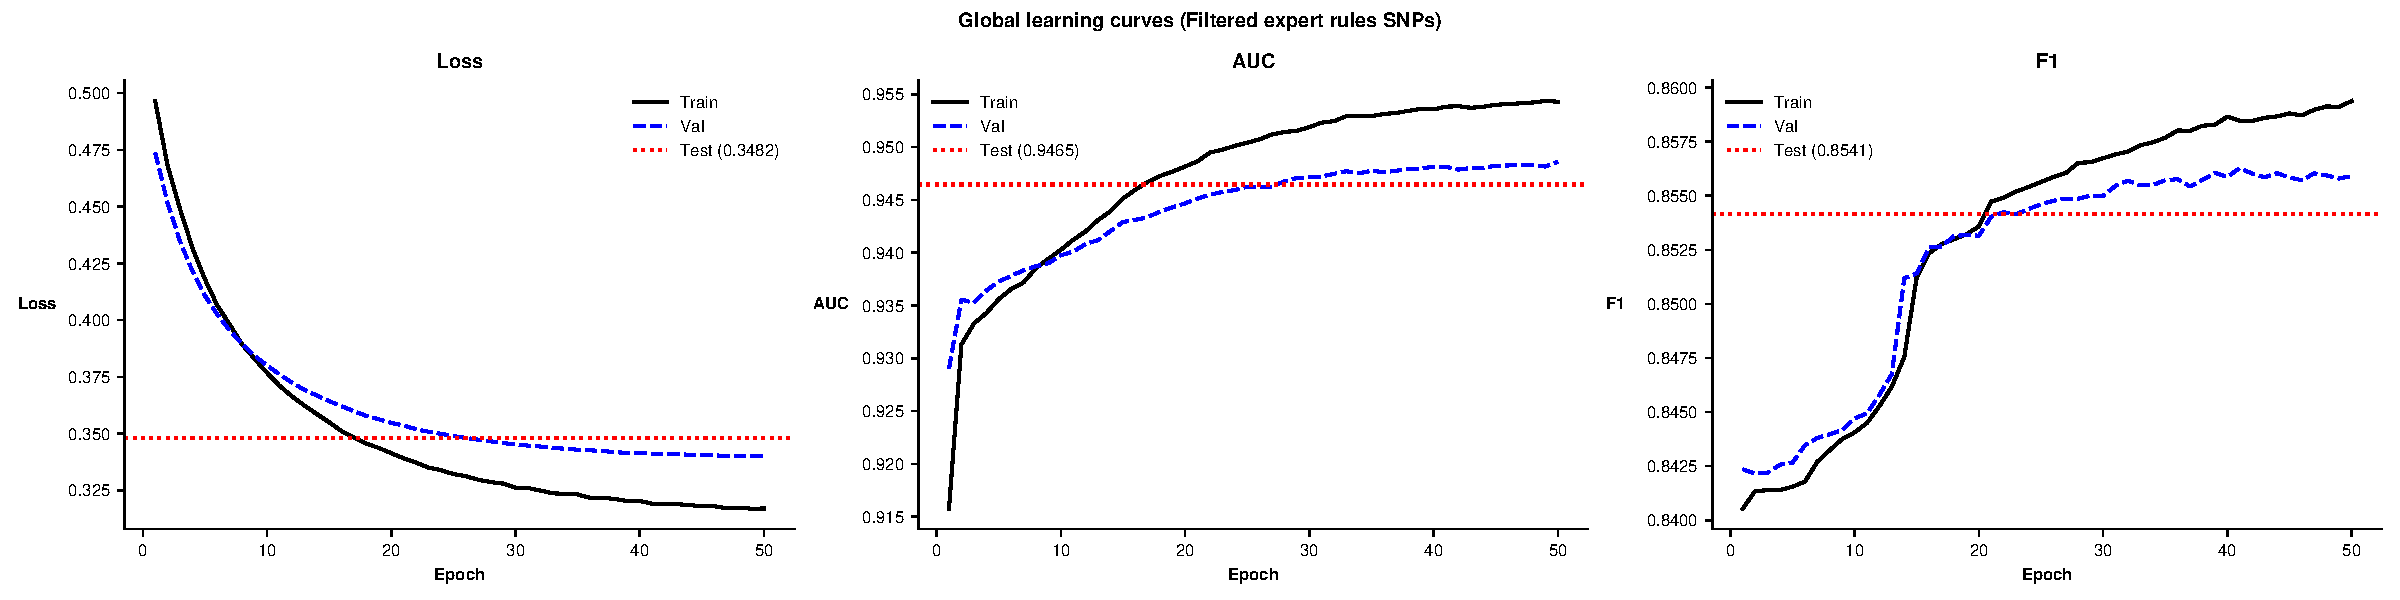
\includegraphics[width=\textwidth]{figures/filtered_expert_rules_learning_curves.pdf}
  \end{center}
  \caption{Global learning curves for er+who catalogue.}\label{fig:filerlr}
\end{figure}

\section{Candidate Mutations}
As per the filtering process outlined in Section [REF], variants from FN samples that were statistically significantly ($-log_{10}(p)>5$) and associated with resistance ($log_{10}(OR)>0$) were selected. Following selection, they were assesed for their inclusion in known lineage markers and in the current ER-updated WHO catalogue scheme. 

Following selection, these variants met two fates: inclusion in what would become WHO+ER+Filtered weight scheme, or for further assessment regarding their candidature as a novel resistance-conferring variant. In this section, for all anti-TB drugs in this dataset, the variants that passed the filtering protocol are displayed in volcano plots in the figures below. The plots are displayed with the $log_{10}(OR)$ in the $x$-axis and the $-log_{10}(p)$ in $y$-axis that were produced during the Fisher's exact test, where the FN samples were `experimental' group and TN the control. The significance and association thresholds are drawn in each plot, creating four quadrants. Top-left houses significant variants not associated with resistance (blue), top-right houses variants that are both associated with resistance and significant (red). Furthermore, the variants the passed the filtering protocols are encircled by a black border (red and black border). Green markers in the graph represent samples with an infinite OR or p-value, due to the variant being present exclusively in resistant or susceptible samples. Variants that produced a sensitivity drop larger than or equal to $5\%$ are annotated, with their gene, polymorphism, and change in sensitivity ($\Delta$Sensitivity). This provides a measurement of the variant's independent predictive contribution, and therefore these variants are of highest priority for validation. The lower left and right quadrants show variants not associated and associated with resistance, but not significant.

Certain volcano plot annotations, and more broadly, filtered variants do not appear to have a name and are deemed the moniker `gene-not-found`. This not suggest an intergenic region, as it has its own annotation, but rather the variant position lacks a human-readable $\texttt{gene=}$ attribute. This tag is common for hypothetical proteins with no assigned gene symbol, \ppe family genes with just a locus tag, and non-coding RNA. This issue can be rectified by locus tag cross-referencing with the TubercuList or PATRIC database [CITE]. They are not discarded as variants in `gene-not-found` locations may be in proximity of genes housing resistance-conferring variants. Resolution of these unknown genes is of high priority for variants that dropped sensitivity steeply post-ablation.

\subsection*{First-line Drugs}

As per Figure~\ref{fig:1st}, the first-line anti-TB agents produced the most-dense plots across all drug classes. Isoniazid, rifampicin, ethambutol and pyrazinamide, displayed many significant variants associated with resistance, highlighted by dense top-right quadrants. Furthermore, on average, the first-line drugs displayed the most outlined variants in the top-right quadrant. 

For isoniazid, the variants that were highlighted from the ablation process were, \textit{katG} C>G, yielding a sensitivity drop of $6.26\%$ when ablated. Furthermore, a `gene not found', a genomic coordinate that is unnamed, had a C>T substitution with a sensitivity drop of $4.56\%$ when ablated. Lastly, an $rpoB$ C>T SNP, in a gene that encodes the drug-target for rifampicin showed an almost borderline decrease in sensitivity of $0.73\%$.

For rifampcin, all annotated variants were located in $rpoB$, the drug-target encoding gene for rifampicin. First of the annotated candidates, $rpoB$ C>T produced a 14.99$\%$ sensitivity drop when ablated. Furthermore, the SNP had approximate $-log_{!0}(p) \approx 120$ and $log_{10}(OR) > 3$, highlighting a 1000-fold enrichment in resistant sample, making it one of the largest sensitivity contributing variants of the first-line drugs. This SNP is followed by $rpoB$ A>T ($\Delta$Sensitivity = 3.37$\%$), $rpoB$ C>G ($\Delta$Sensitivity = 1.22$\%$) and $rpoG$ C>T (different position) ($\Delta$Sensitivity = 1.26$\%$) which is denoted by green box.

Ethambutol yielded the most diverse set of ablated variants of the first line drugs. All annotated variants were in $embB$, drug-target encoding gene for Ethambutol, which is an arabinosyltransferase, essential for arabionogalactan synthesis [CITE]. The filtered variants that met or exceeded the sensitivity-drop threshold were $embB$ A>G (Position= 4247429, $\Delta$Sensitivity= 2.56$\%$, FNP= 95$\%$, RSM= 2$\%$), A>G (Position = 4247847, $\Delta$Sensitivity= 0.66$\%$, FNP= 90$\%$, RSM= 2$\%$), G>C ($\Delta$Sensitivity= 0.97$\%$, FNP= 80$\%$, RSM= 2$\%$), G>A ($\Delta$Sensitivity= 1.05$\%$, FNP=) and A>C ($\Delta$Sensitivity= 1.77$\%$, FNP= 100$\%$, RSM= 2$\%$, green marker) (Figure, Table). Two highly significant SNPs $rpoB$ C>T ($\Delta$Sensitivity= 2.33$\%$) and $katG$ C>G ($\Delta$Sensitivity= 0.97$\%$) were observed. These are likely confounders as the gene products of $rpoB$ or $katG$ are not involved in ethambutol's mechanism of action. Although they are highly significant (p-values $\sim 10^{-140}$) compared to $embB$ variants ($5 \leq$ p-values $\leq 60$), they have relatively modest association with ethambutol resistance (10-fold associated with resistance compared to $embB \geq 10$ with resistance). Additionally, variants in the \ppe gene family were observed with variants in $PE-PGRS$4, 6, 7, 9, and 19 and $PPE$54, 55, and 60 (Table).

To conclude the first-line drugs, pyrazinamide did not produce any ablated variants that passed the sensitivity-loss threshold. However, pyrazinamide produced a large, densely populated plot with many significant variants with positive associations (Figure~\ref{fig:1st}). This can be observed in the filtered variants, where in the pyrazinamide FN samples, the novel variants were in the \ppe family. Variants in $PPE$54, 55 and 60, and $PE-PGRS$4 and 9 can be observed (Table). 

\begin{figure}[H]
    \centering
    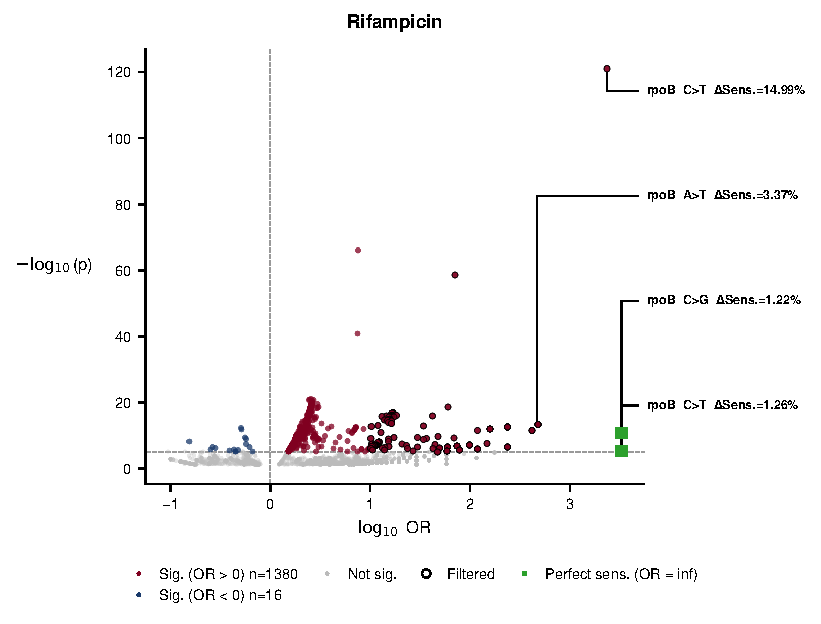
\includegraphics[width=0.45\textwidth]{./figures/plots/rifampicin_volcano.pdf}
    \hfill
    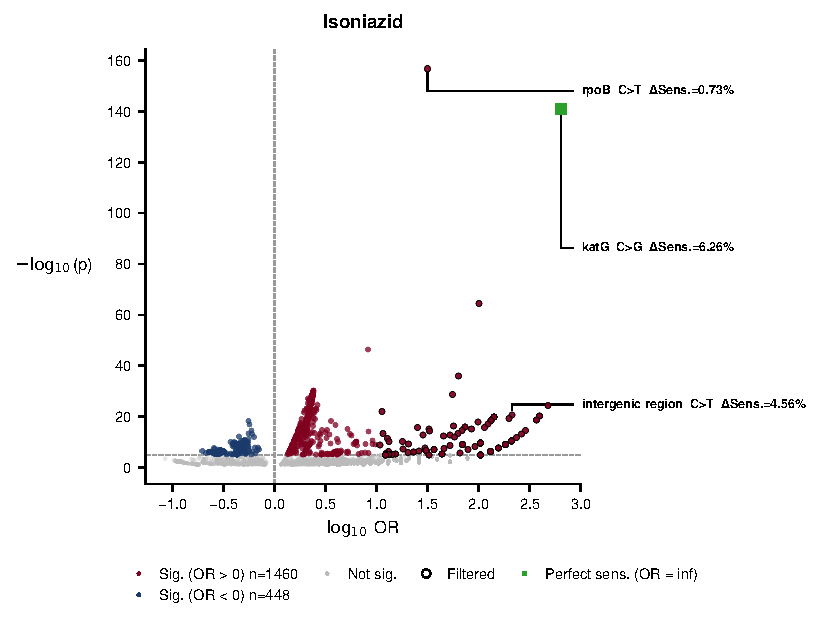
\includegraphics[width=0.45\textwidth]{./figures/plots/isoniazid_volcano.pdf}
    \hfill
    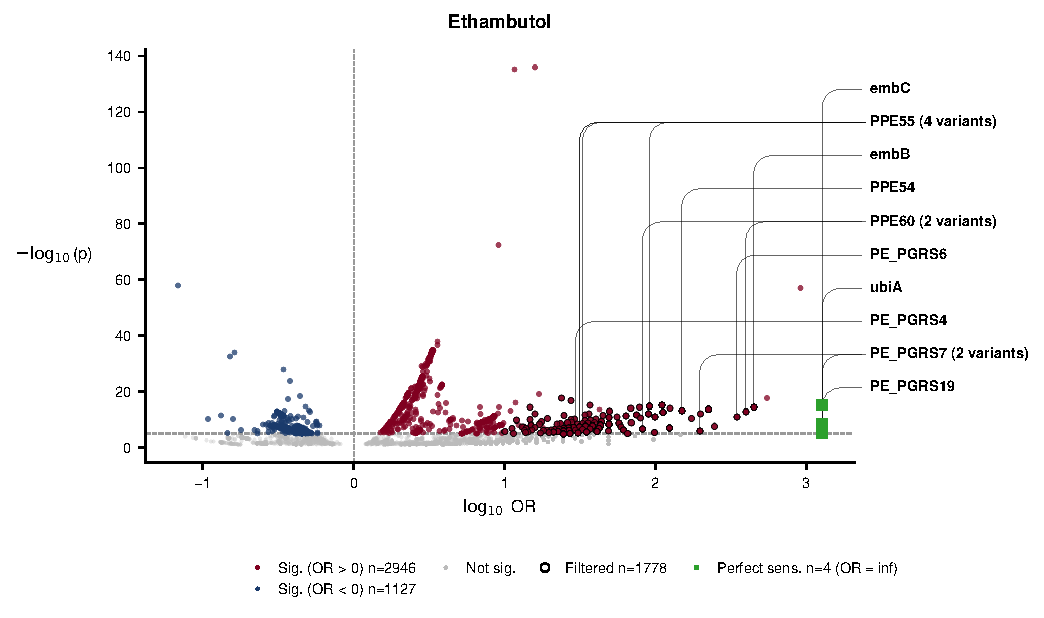
\includegraphics[width=0.45\textwidth]{./figures/plots/ethambutol_volcano.pdf}
    \hfill
    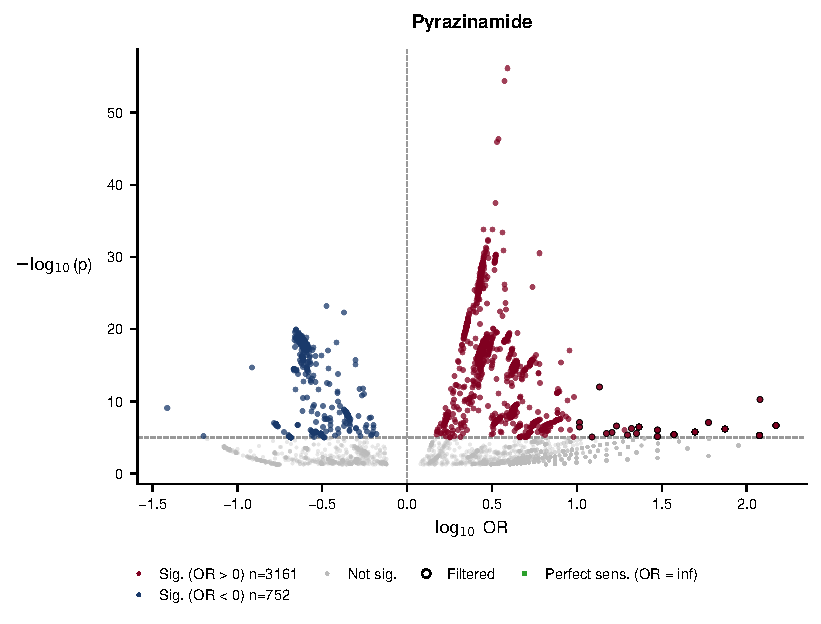
\includegraphics[width=0.45\textwidth]{./figures/plots/pyrazinamide_volcano.pdf}
    \hfill
  \label{fig:1st}
\end{figure}

\subsection{Second-line Drugs}

\subsubsection{Group A}

\begin{figure}[H]
    \centering
    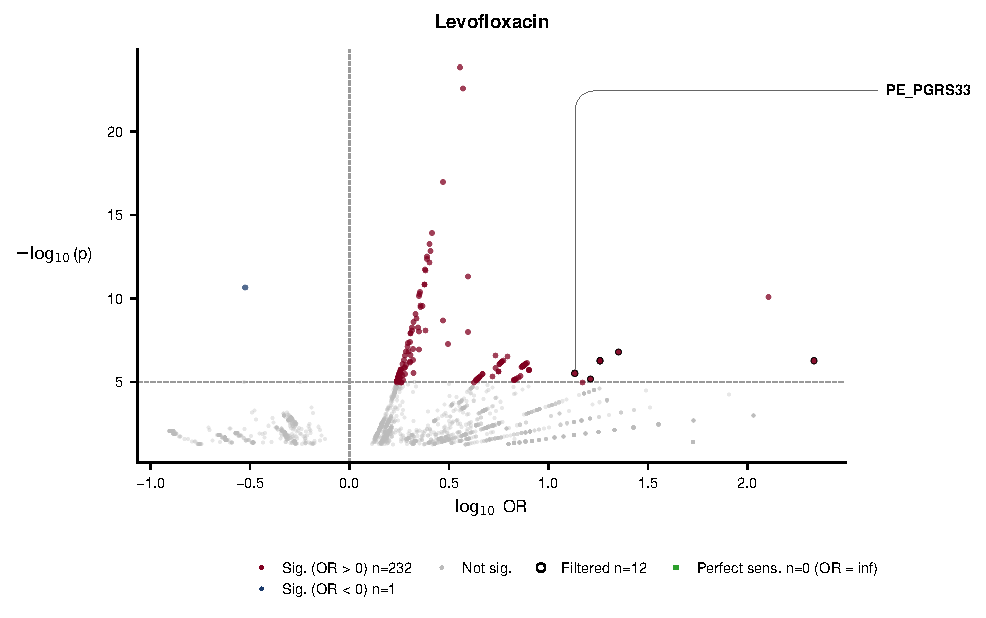
\includegraphics[width=0.45\textwidth]{./figures/plots/levofloxacin_volcano.pdf}
    \hfill
    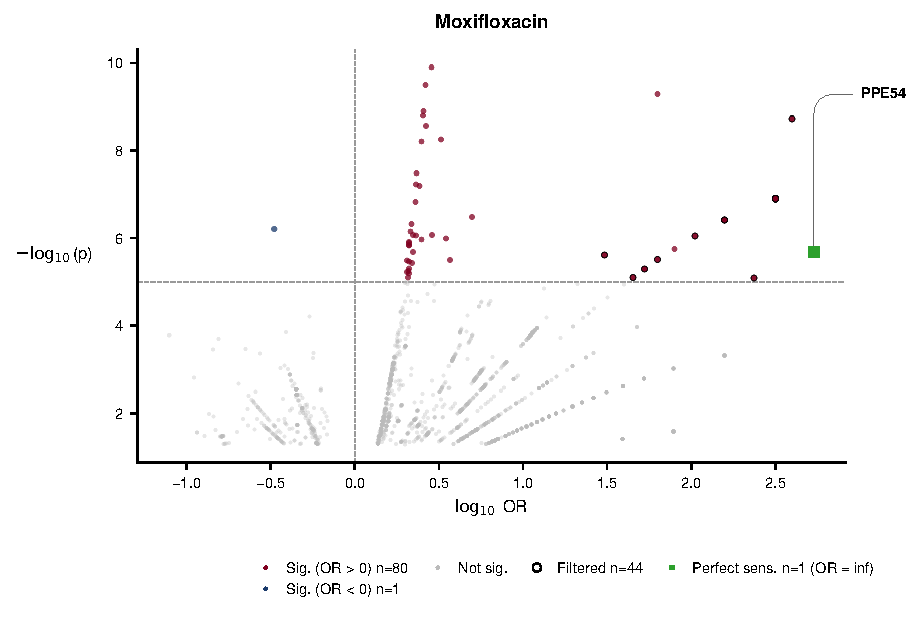
\includegraphics[width=0.45\textwidth]{./figures/plots/moxifloxacin_volcano.pdf}
    \hfill
    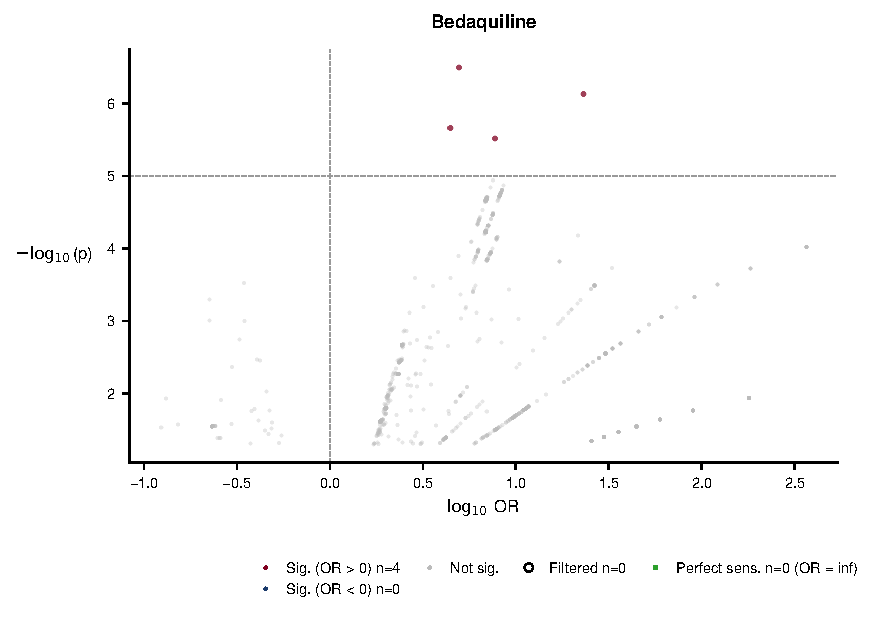
\includegraphics[width=0.45\textwidth]{./figures/plots/bedaquiline_volcano.pdf}
    \hfill
    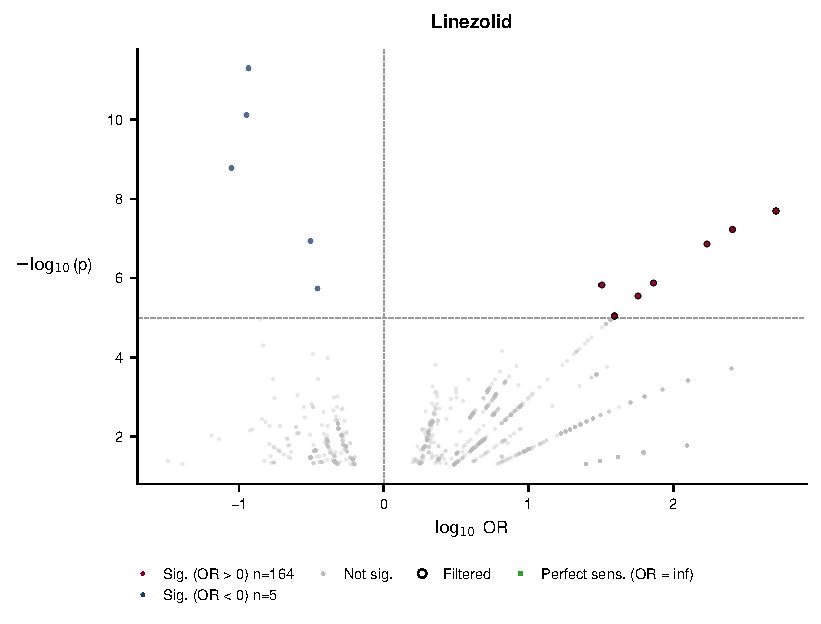
\includegraphics[width=0.45\textwidth]{./figures/plots/linezolid_volcano.pdf}
    \hfill
\end{figure}

\subsubsection{Group B}

Clofazimine unknown mutation is in Rv3254, a conserved hypothetical protein \cite{minato2019genomewide}.

\begin{figure}[H]
    \centering
    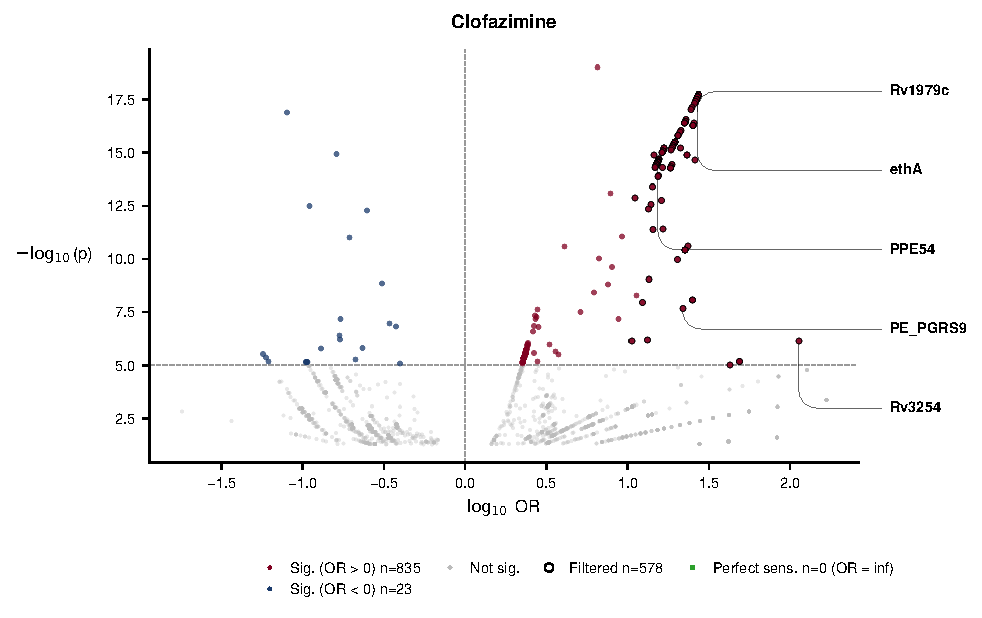
\includegraphics[width=0.45\textwidth]{./figures/plots/clofazimine_volcano.pdf}
    \hfill
    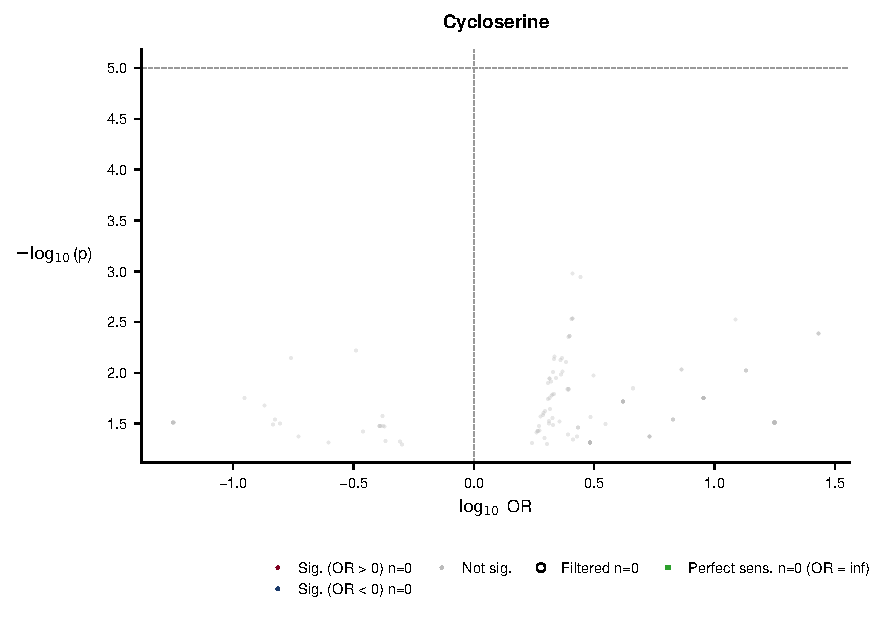
\includegraphics[width=0.45\textwidth]{./figures/plots/cycloserine_volcano.pdf}
    \hfill
\end{figure}

\subsubsection{Group C}

The gene-not-found for ethionamide is the same for isoniazid, 14bp upstream of $fabG1$, which makes sense biologically, since there's cross-resistance \cite{valafar2021systematic}. 

\begin{figure}[H]
    \centering
    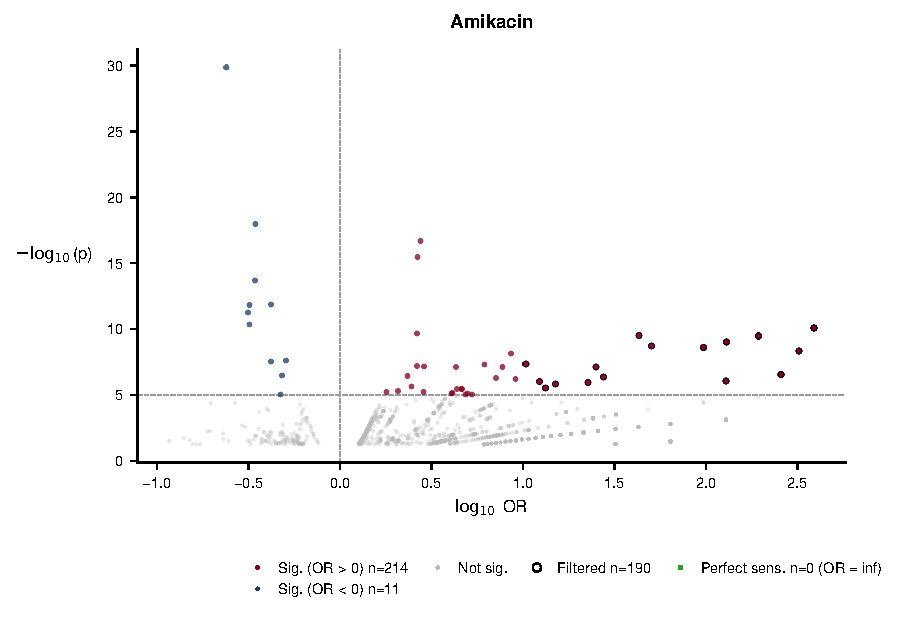
\includegraphics[width=0.45\textwidth]{./figures/plots/amikacin_volcano.pdf}
    \hfill
    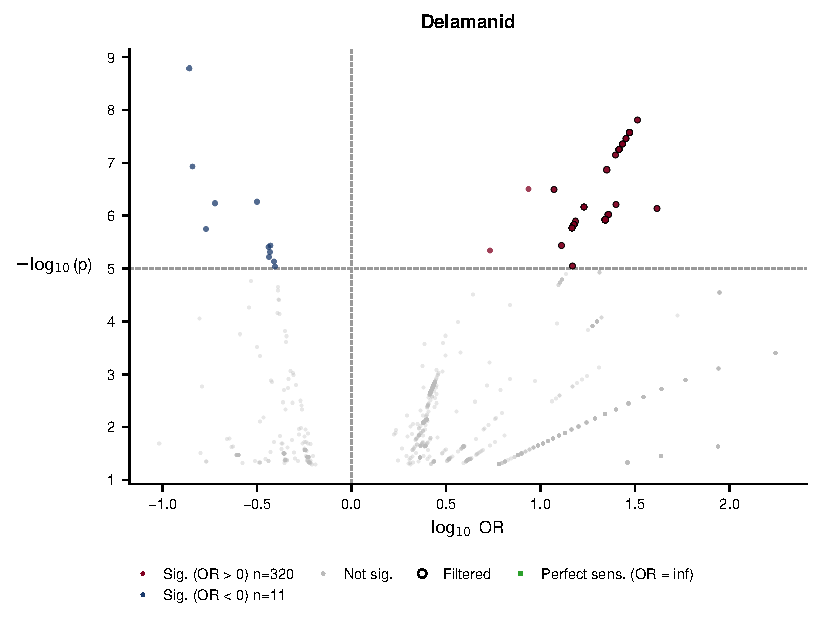
\includegraphics[width=0.45\textwidth]{./figures/plots/delamanid_volcano.pdf}
    \hfill
    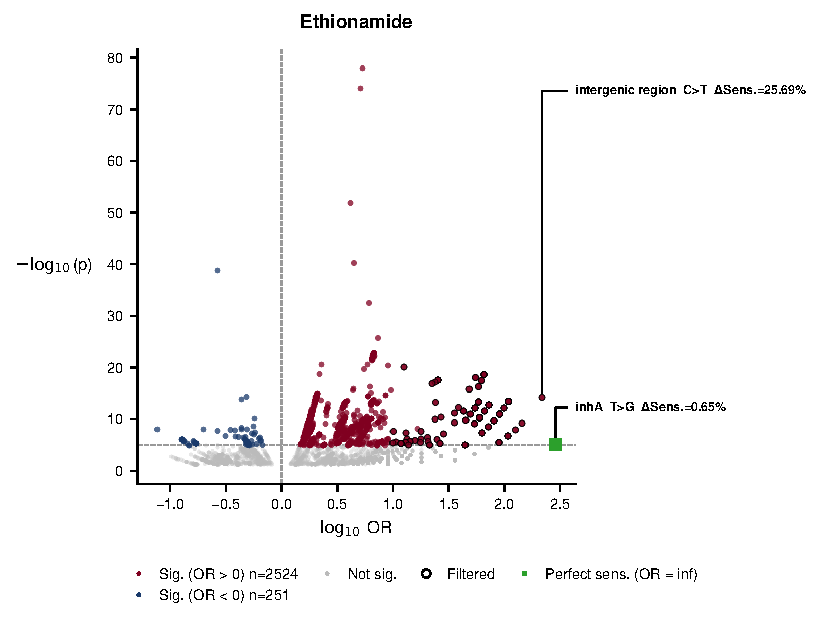
\includegraphics[width=0.45\textwidth]{./figures/plots/ethionamide_volcano.pdf}
    \hfill
    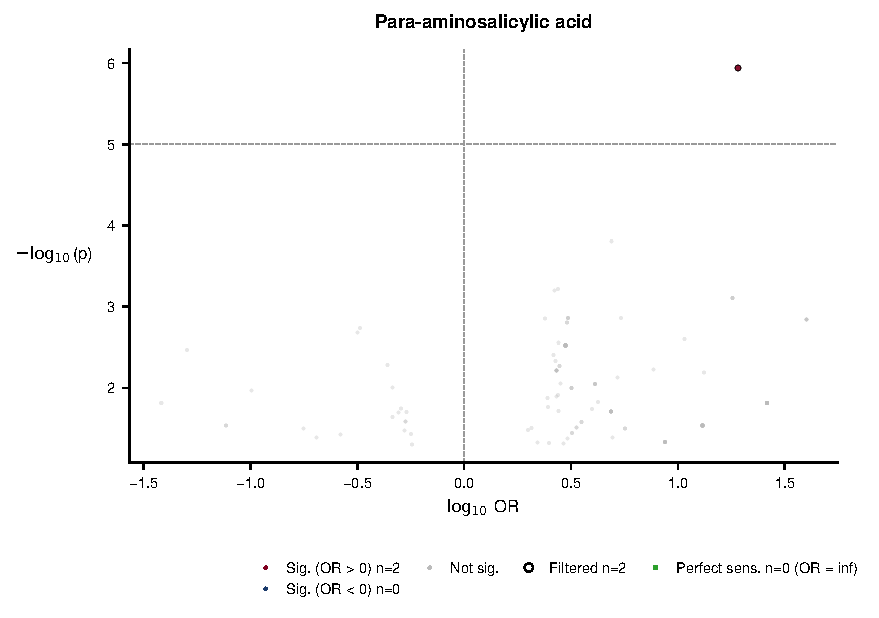
\includegraphics[width=0.45\textwidth]{./figures/plots/para-aminosalicylic_acid_volcano.pdf}
    \hfill
\end{figure}

\subsection{Other drugs}


\begin{figure}[H]
    \centering
    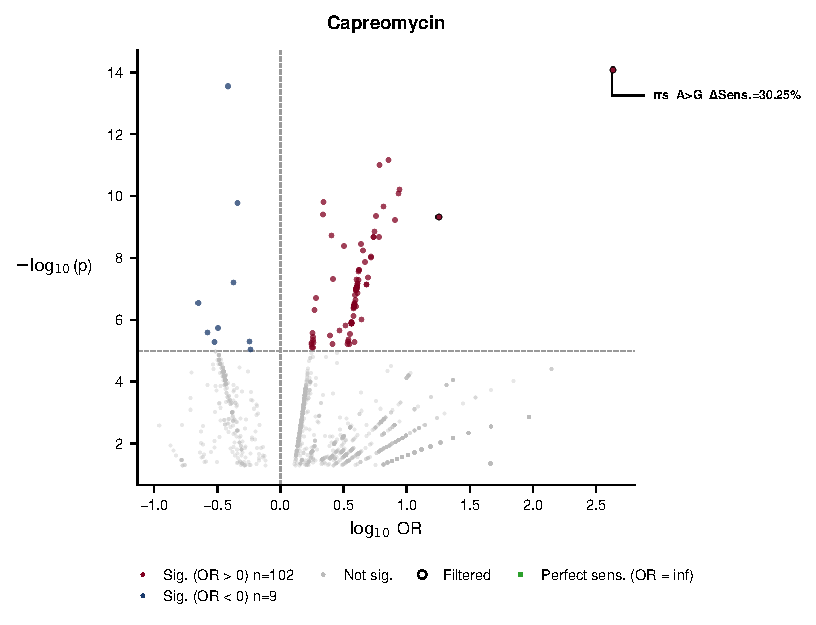
\includegraphics[width=0.45\textwidth]{./figures/plots/capreomycin_volcano.pdf}
    \hfill
    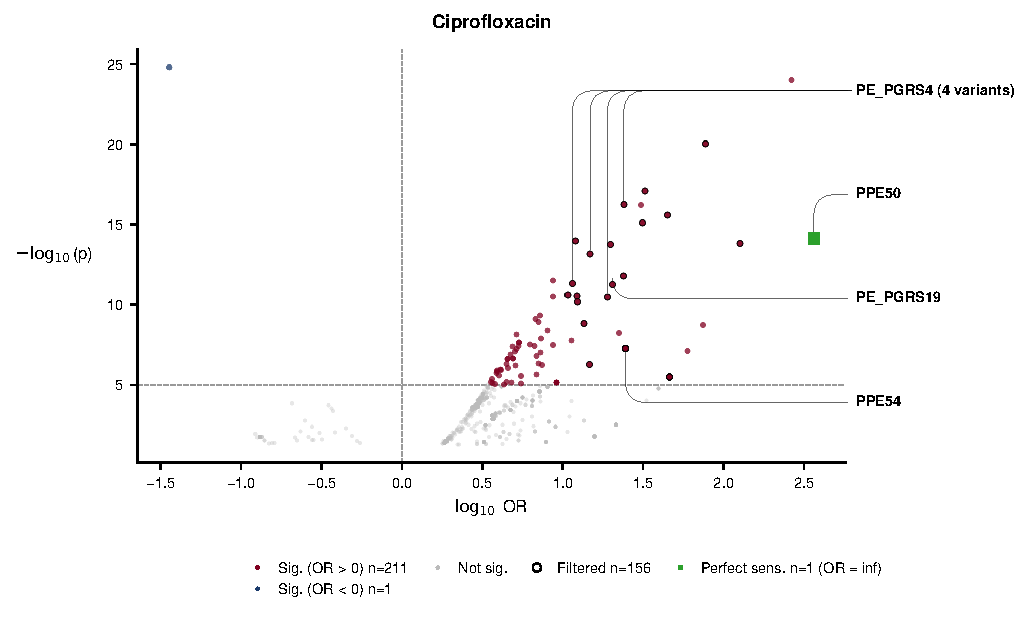
\includegraphics[width=0.45\textwidth]{./figures/plots/ciprofloxacin_volcano.pdf}
    \hfill
    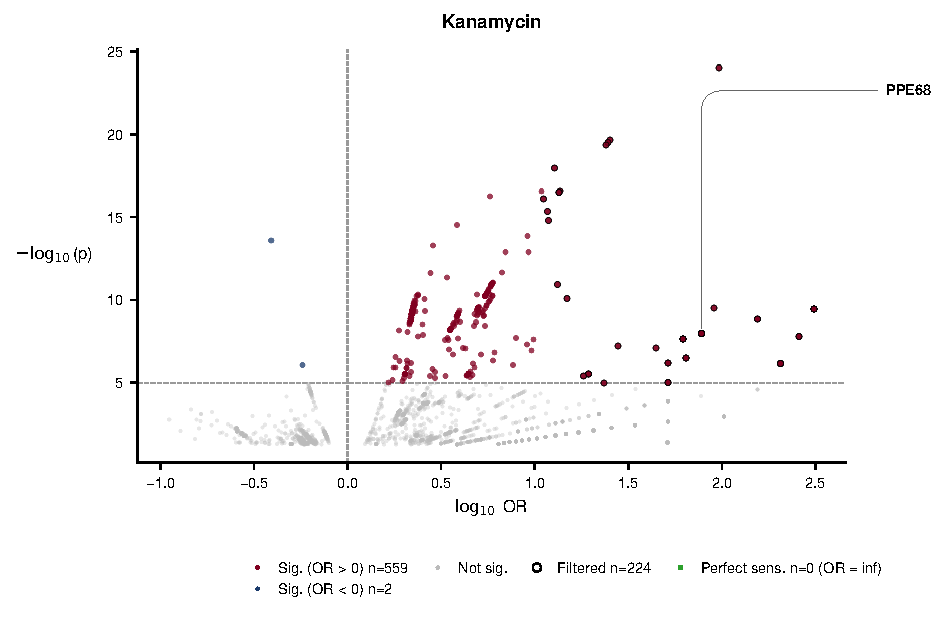
\includegraphics[width=0.45\textwidth]{./figures/plots/kanamycin_volcano.pdf}
    \hfill
    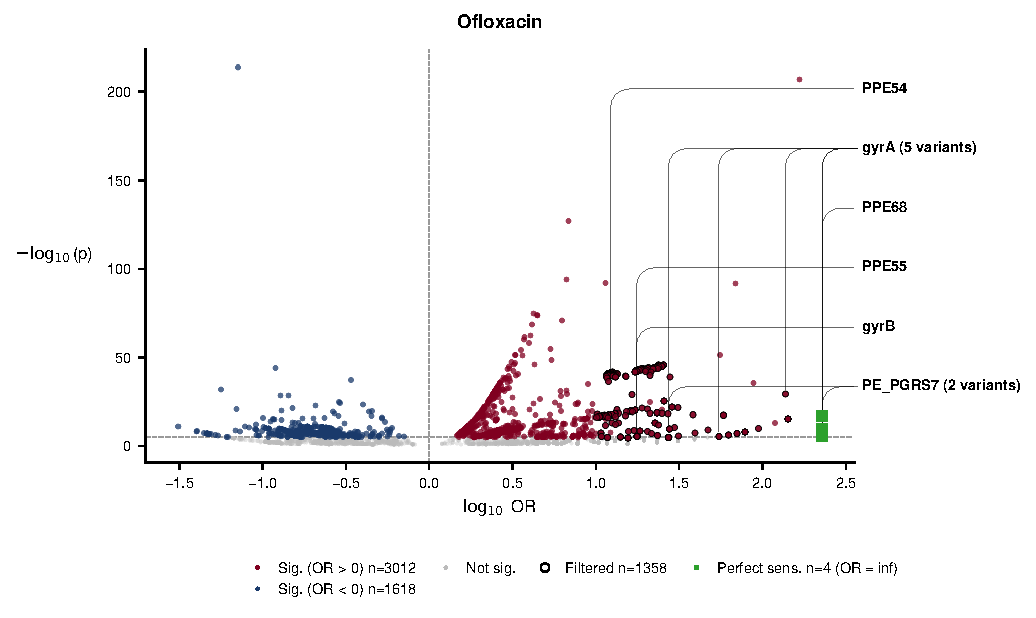
\includegraphics[width=0.45\textwidth]{./figures/plots/ofloxacin_volcano.pdf}
    \hfill
\end{figure}

\input{Chapters/Results/tb_tab.tex}


\graphicspath{{Figures/Discussion}}

\chapter{Discussion}\label{ch:discc}
\begin{itemize}
  \item \textbf{The Reminder:} Re-state the core biological/computational problem your thesis tackled
  \item \textbf{The Headline Finding:} State your absolute biggest achievement without listing a wall of specific metrics.
  \item \textbf{The Executive "Why":} Give a one-sentence conceptual reason for your success.
\end{itemize}

\section{Model Performance}
\begin{itemize}
  \item Why are they this way? Explain the mechanics behind the scores
  \item Where does it fit? Compare this to the literature.
\end{itemize}

\section{Ablation Study and Biological Significance}
\begin{itemize}
  \item Why are they this way? Explain the mechanics behind the scores
  \item Where does it fit? Compare this to the literature.
\end{itemize}

\section{Candidate Variants}

The $katG$ C>G SNP has biological grounding, as $katG$ encodes a catalase-peroxidase that activates the prodrug for isoniazid [CITE]. With non-synonymous variants in $katG$ being a substantial reservoir for resistance-conferring variants in clinical samples, an uncatalogued variant that is both significant and associated with resistance, and produced a $-6.26\%$ change in sensitivity when ablated poses as a high-priority variant warranting further characterisation and investigation.  

The `gene-not-found' C>T variant also showed a considerable drop in sensitivity of $4.56\%$, and has potential for investigation as a resistance-marker. This variant is located 14bp upstream of $fabG1$, an enzyme involved in mycolic acid biosynthesis, and more importantly, a gene that contains resistance-conferring variants for isoniazid and ethionamide \cite{valafar2021systematic}. Given an approximate 5$\%$ sensitivity dip post-ablation, and proximity to $fabG1$, this variant warrants further investigation. 

Lastly, an $rpoB$ C>T SNP yielded a drop in sensitivity of 0.73$\%$. This is very likely a confounder, as $rpoB$ encodes the $\beta$ subunit of RNA polymerase [CITE], which is the target for rifampicin. This appearance is likely because MDR-TB strains carry resistance to both rifampicin and isoniazid. Future weight matrix revisions for isoniazid warrants removal to prevent FPs. 

This validates our internal pipelines, which identified the correct gene and location. The enrichment of $rpoB$ C>T annotated SNP, is one of the strongest candidates for validation from the FN subset. All $rpoB$ variants close to, or within RRDR (codons 426-452). 


Multiple SNPs at distinct positions, indicates possible diverse resistant variants over a single dominant mutation. This is consistent with literature surrounding clincinal ethambutol resistance which report a wide spectrum of $embB$ variants. These candidates are of high-priority for validation. Furthermore, variants appeared in auxiliary genes involved in $embB$ resistance such as $embC$ and $ubiA$.
\section{Limitations}
\begin{itemize}
  \item Why are they this way? Explain the mechanics behind the scores
  \item Where does it fit? Compare this to the literature.
\end{itemize}
\section{Future Studies}
\begin{itemize}
  \item Why are they this way? Explain the mechanics behind the scores
  \item Where does it fit? Compare this to the literature.
\end{itemize}

 
\singlespacing


% ********************************************************************
% Backmatter
%*******************************************************
% Bibliography
\cleardoublepage
% Bibliography
%*******************************************************
\clearpage
\phantomsection

% 1. Set running page headers manually using standard LaTeX syntax
\markboth{REFERENCES}{REFERENCES}

% 2. Add the bibliography to your Table of Contents
\addcontentsline{toc}{chapter}{References}

% 3. Print the actual Chapter Title on the page using a clean style
\chapter*{References}

% 4. Print the references in scriptsize using a plain heading style
\begingroup
  \fontsize{8}{10}\selectfont 
  \printbibliography[heading=none] % Completely bypasses all broken template headers
\endgroup


% Appendix
\appendix
% \renewcommand{\thechapter}{\alph{chapter}}
\cleardoublepage
% \part*{Appendix}
\chapter{Appendix A}
\begin{figure}[H]
  \begin{center}
    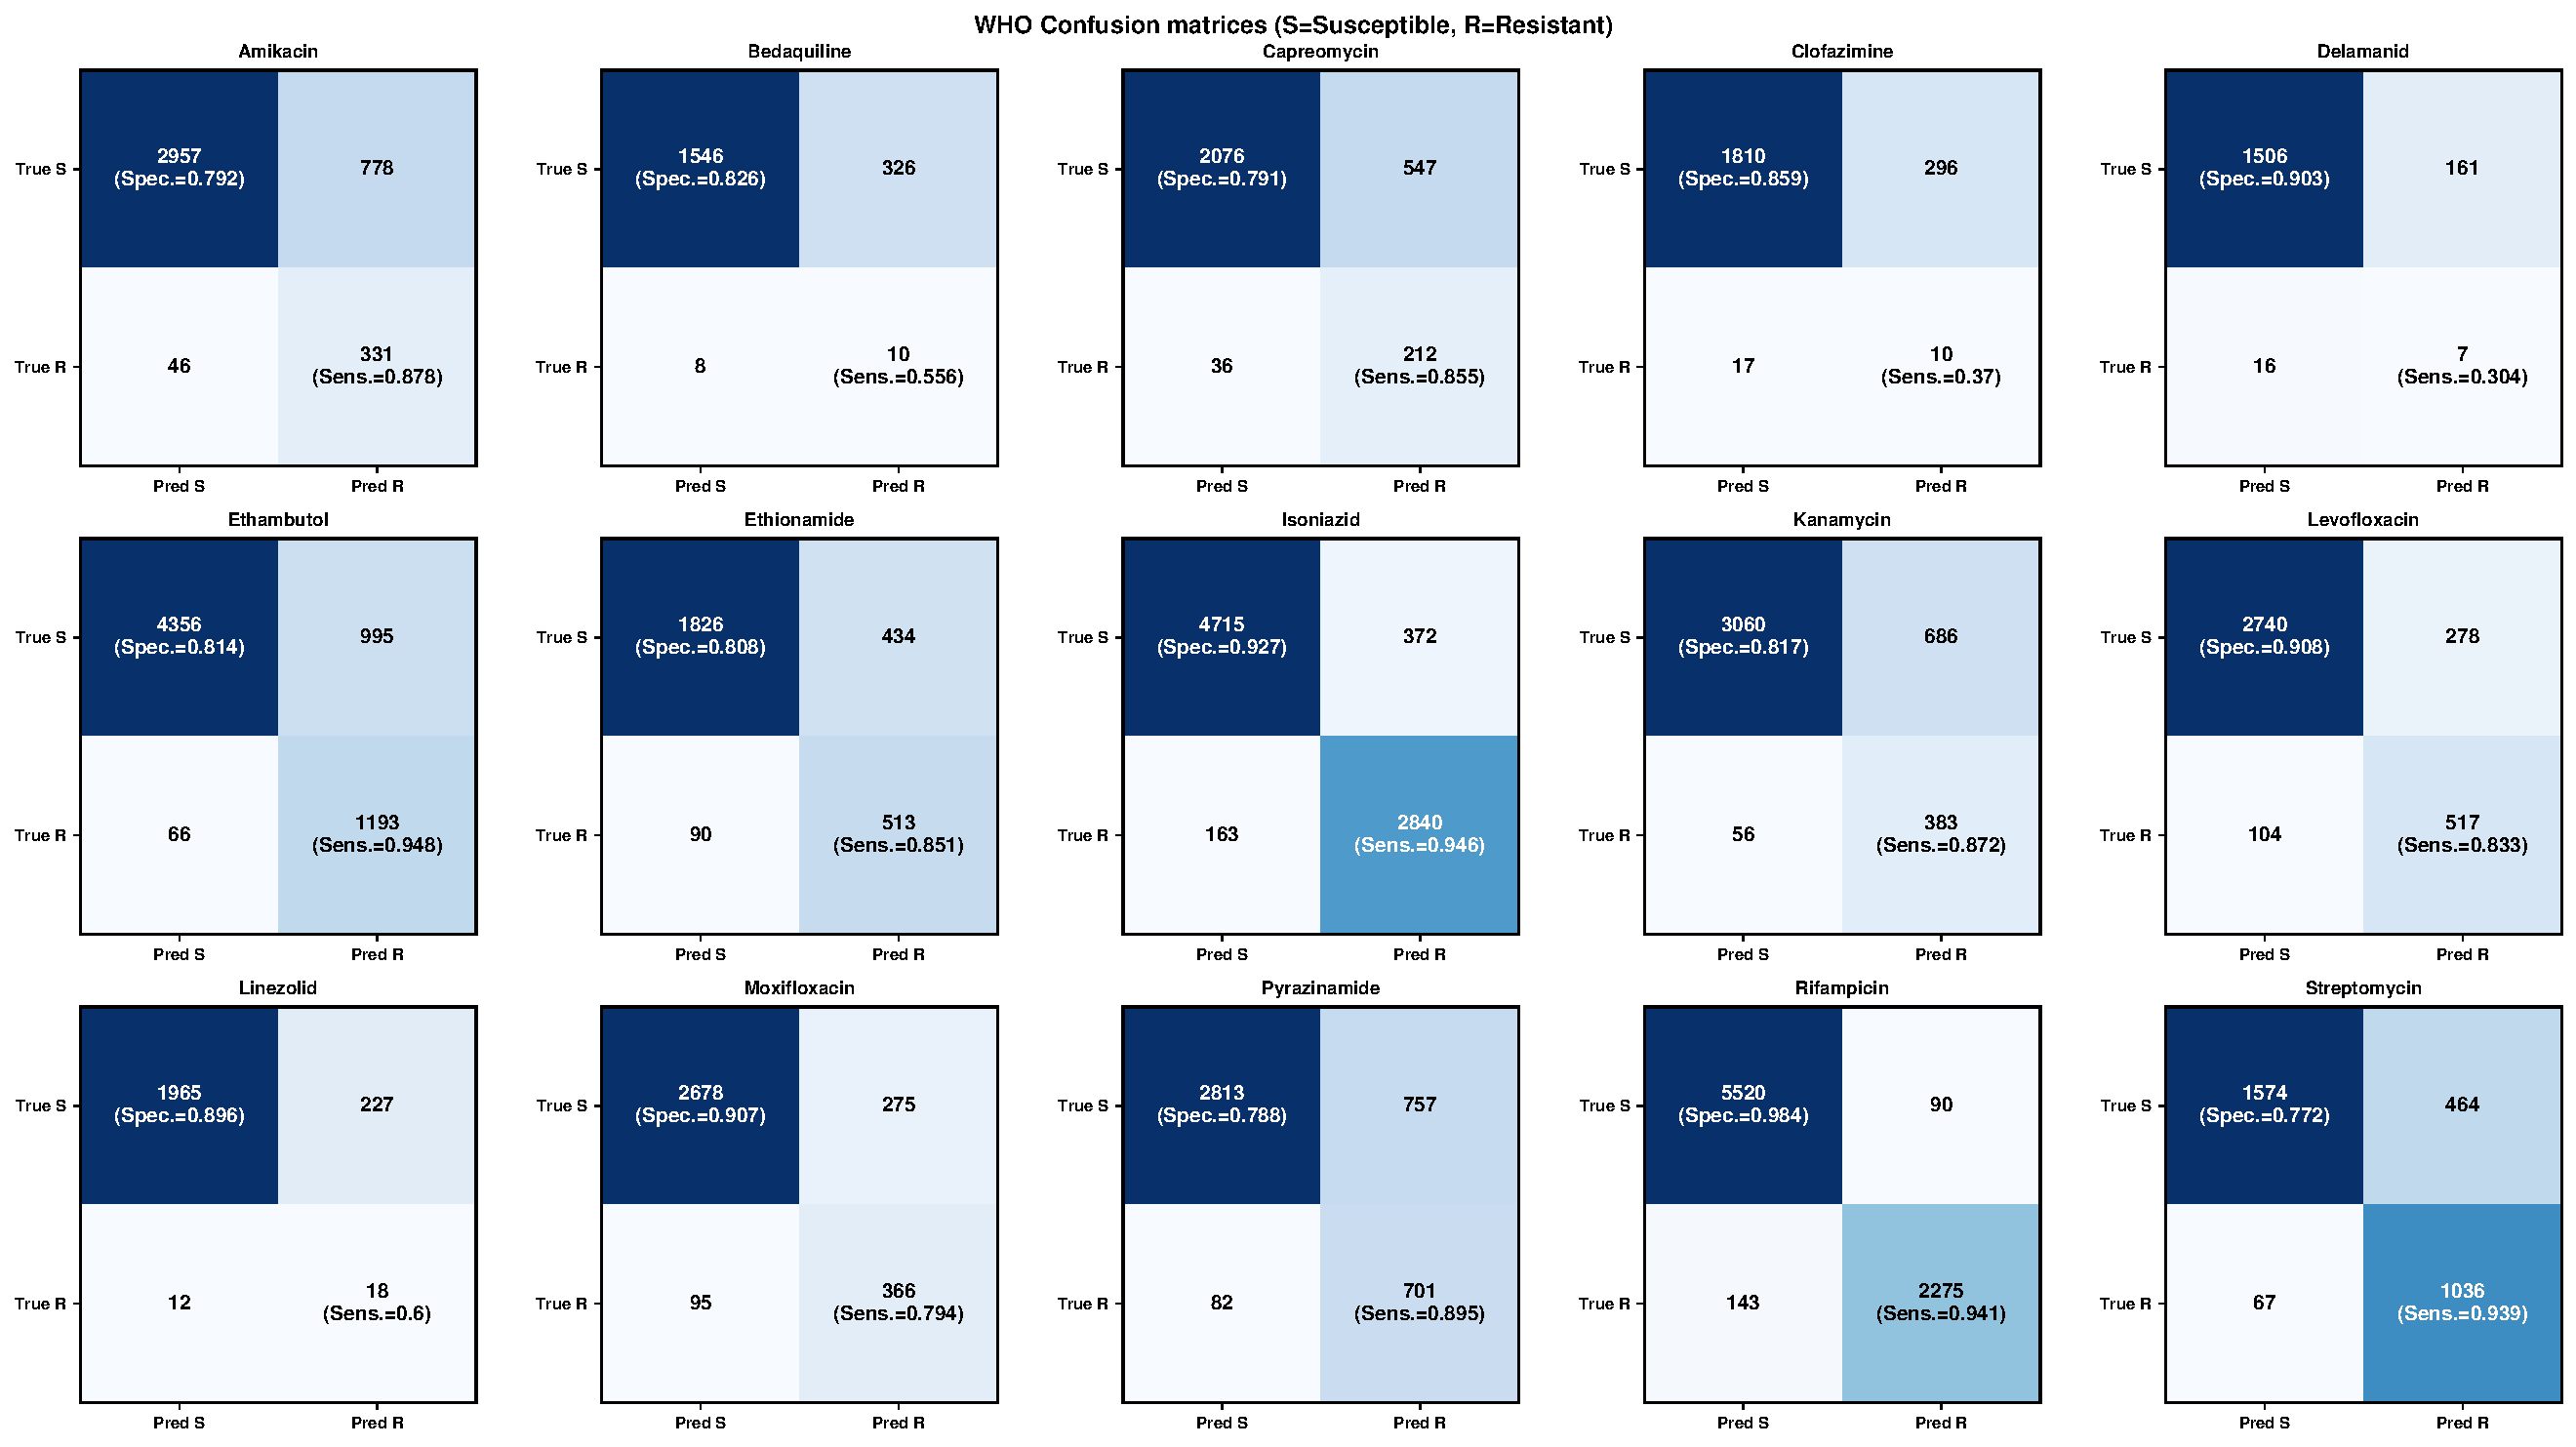
\includegraphics[width=\textwidth]{figures/who_confusion_matrices.pdf}
  \end{center}
  \caption{Confusion matrix for 16 drugs for the WHO snp catalogue}\label{fig:whocm}
\end{figure}

\begin{figure}[H]
  \begin{center}
    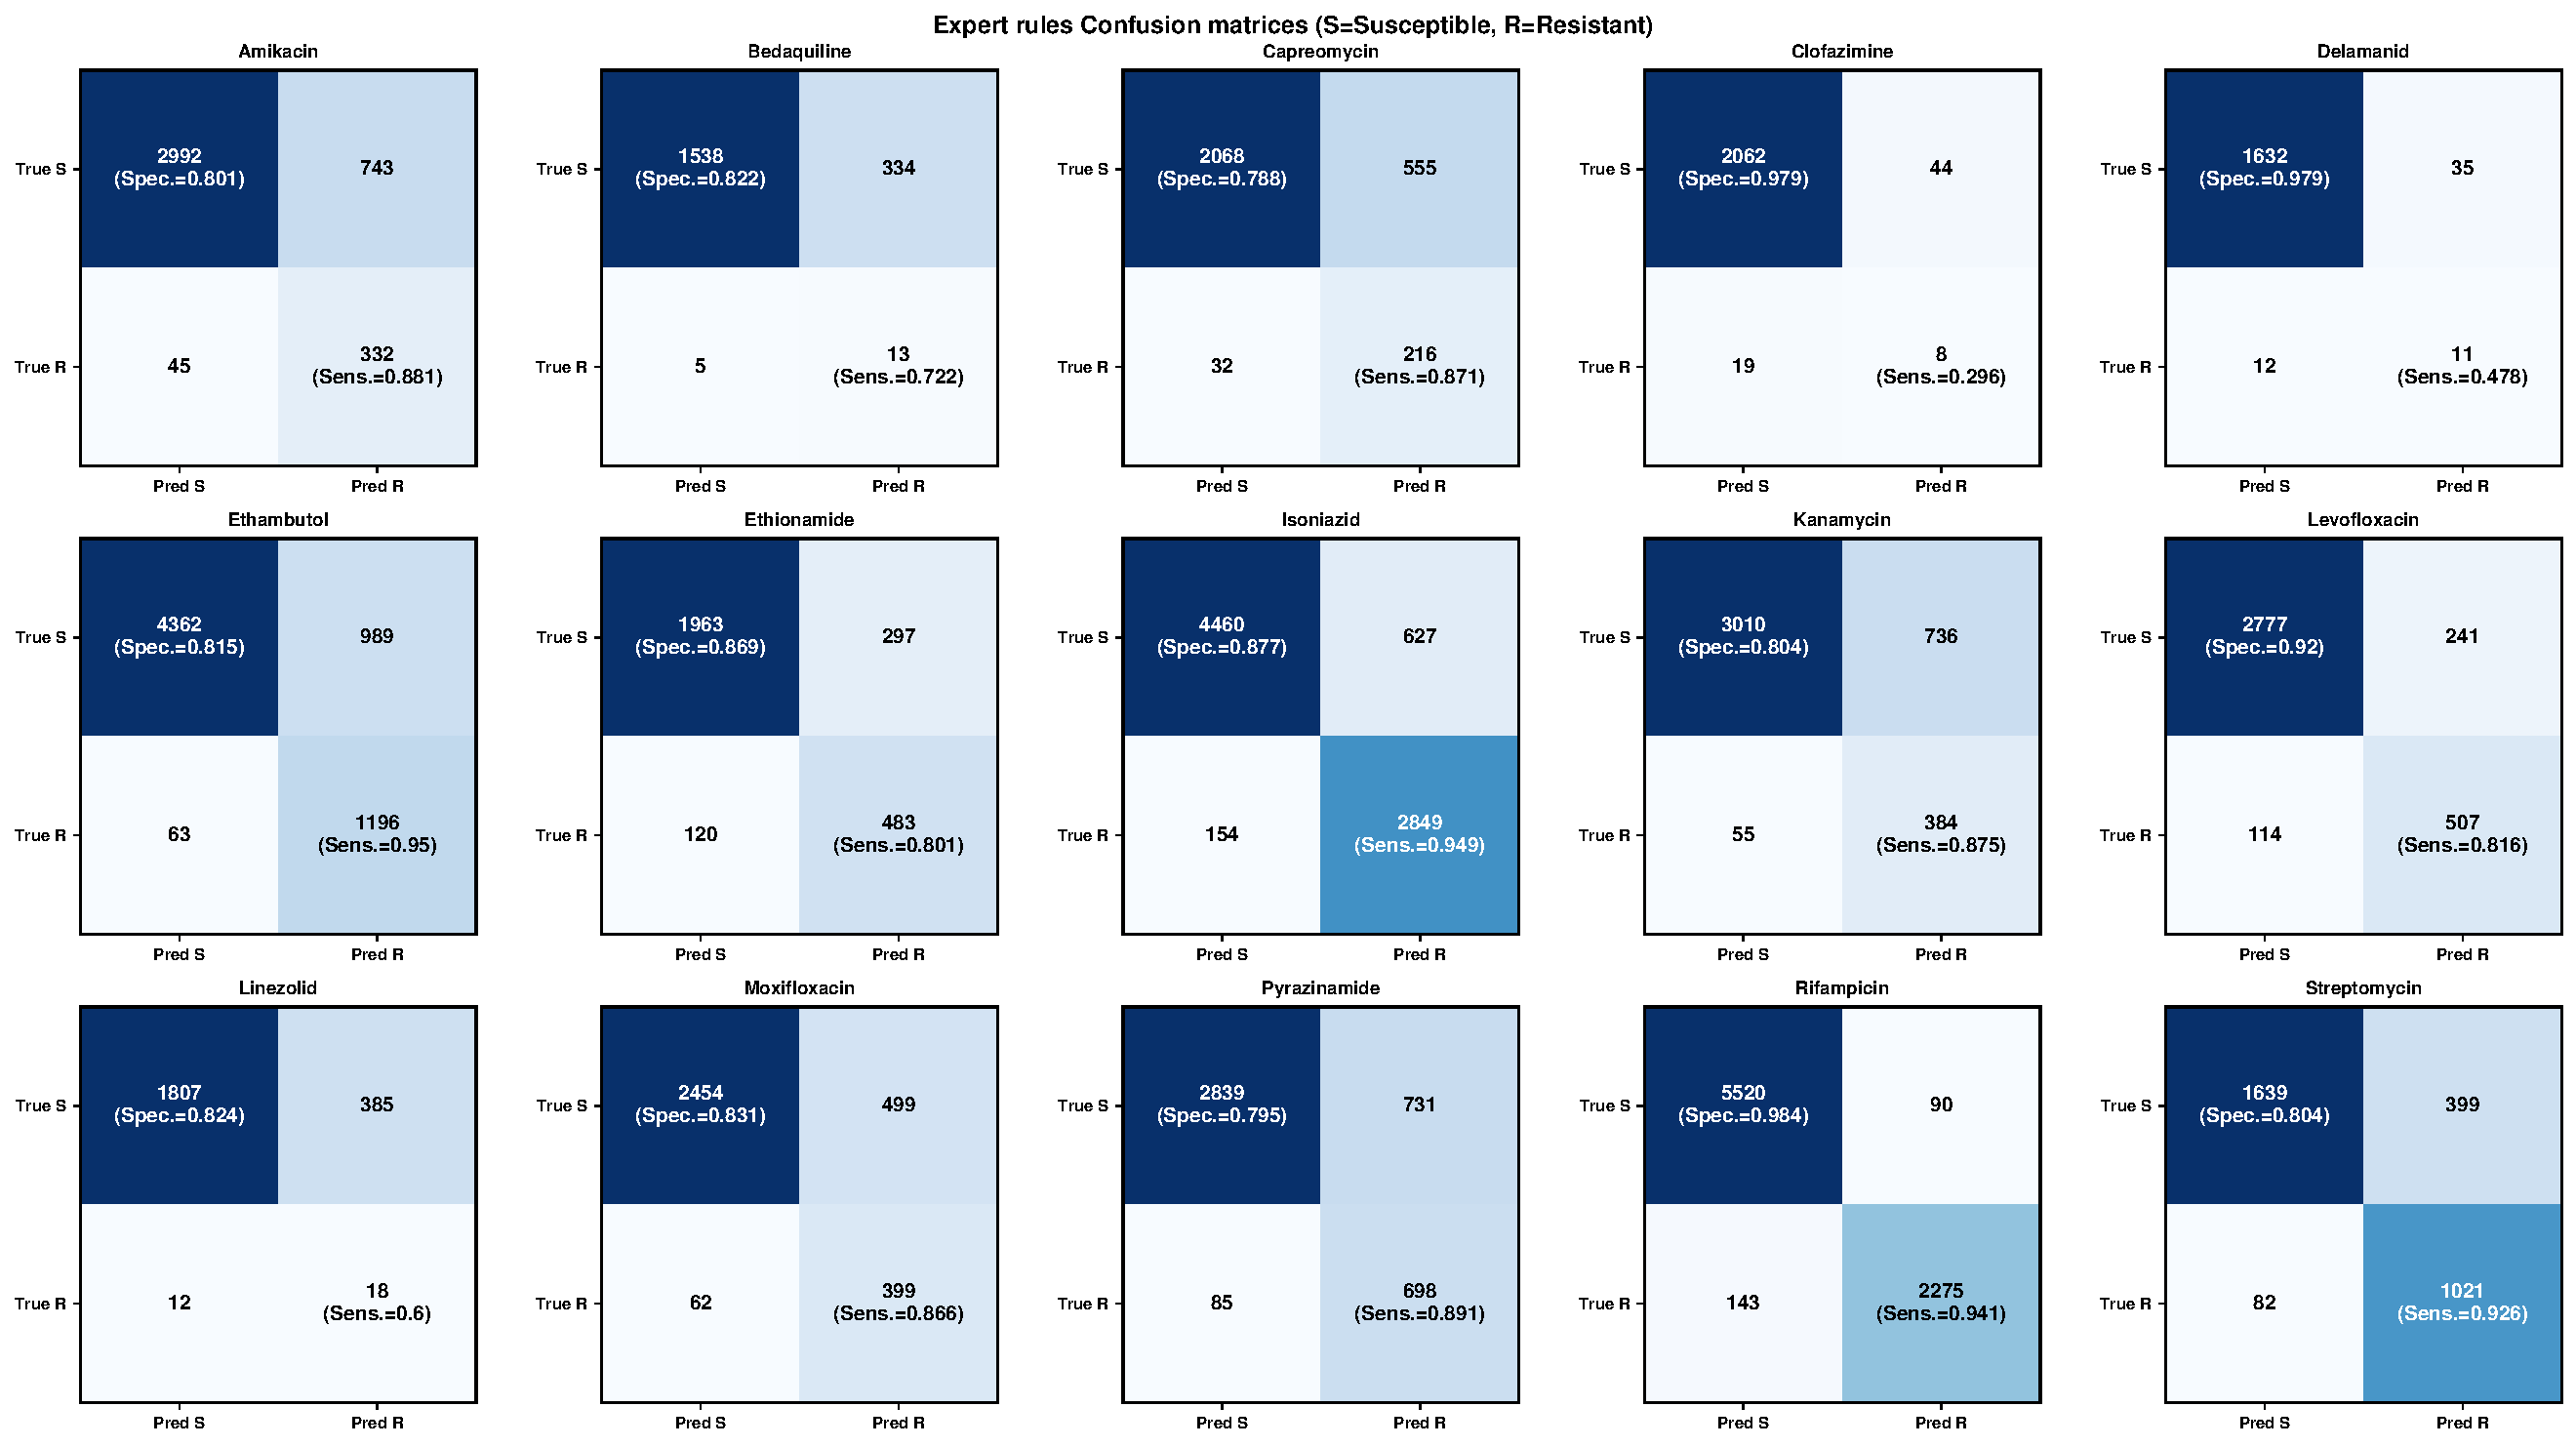
\includegraphics[width=\textwidth]{figures/expert_rules_confusion_matrices.pdf}
  \end{center}
  \caption{Confusion matrix for er+who catalogue.}\label{fig:ercm}
\end{figure}

\begin{figure}[H]
  \begin{center}
    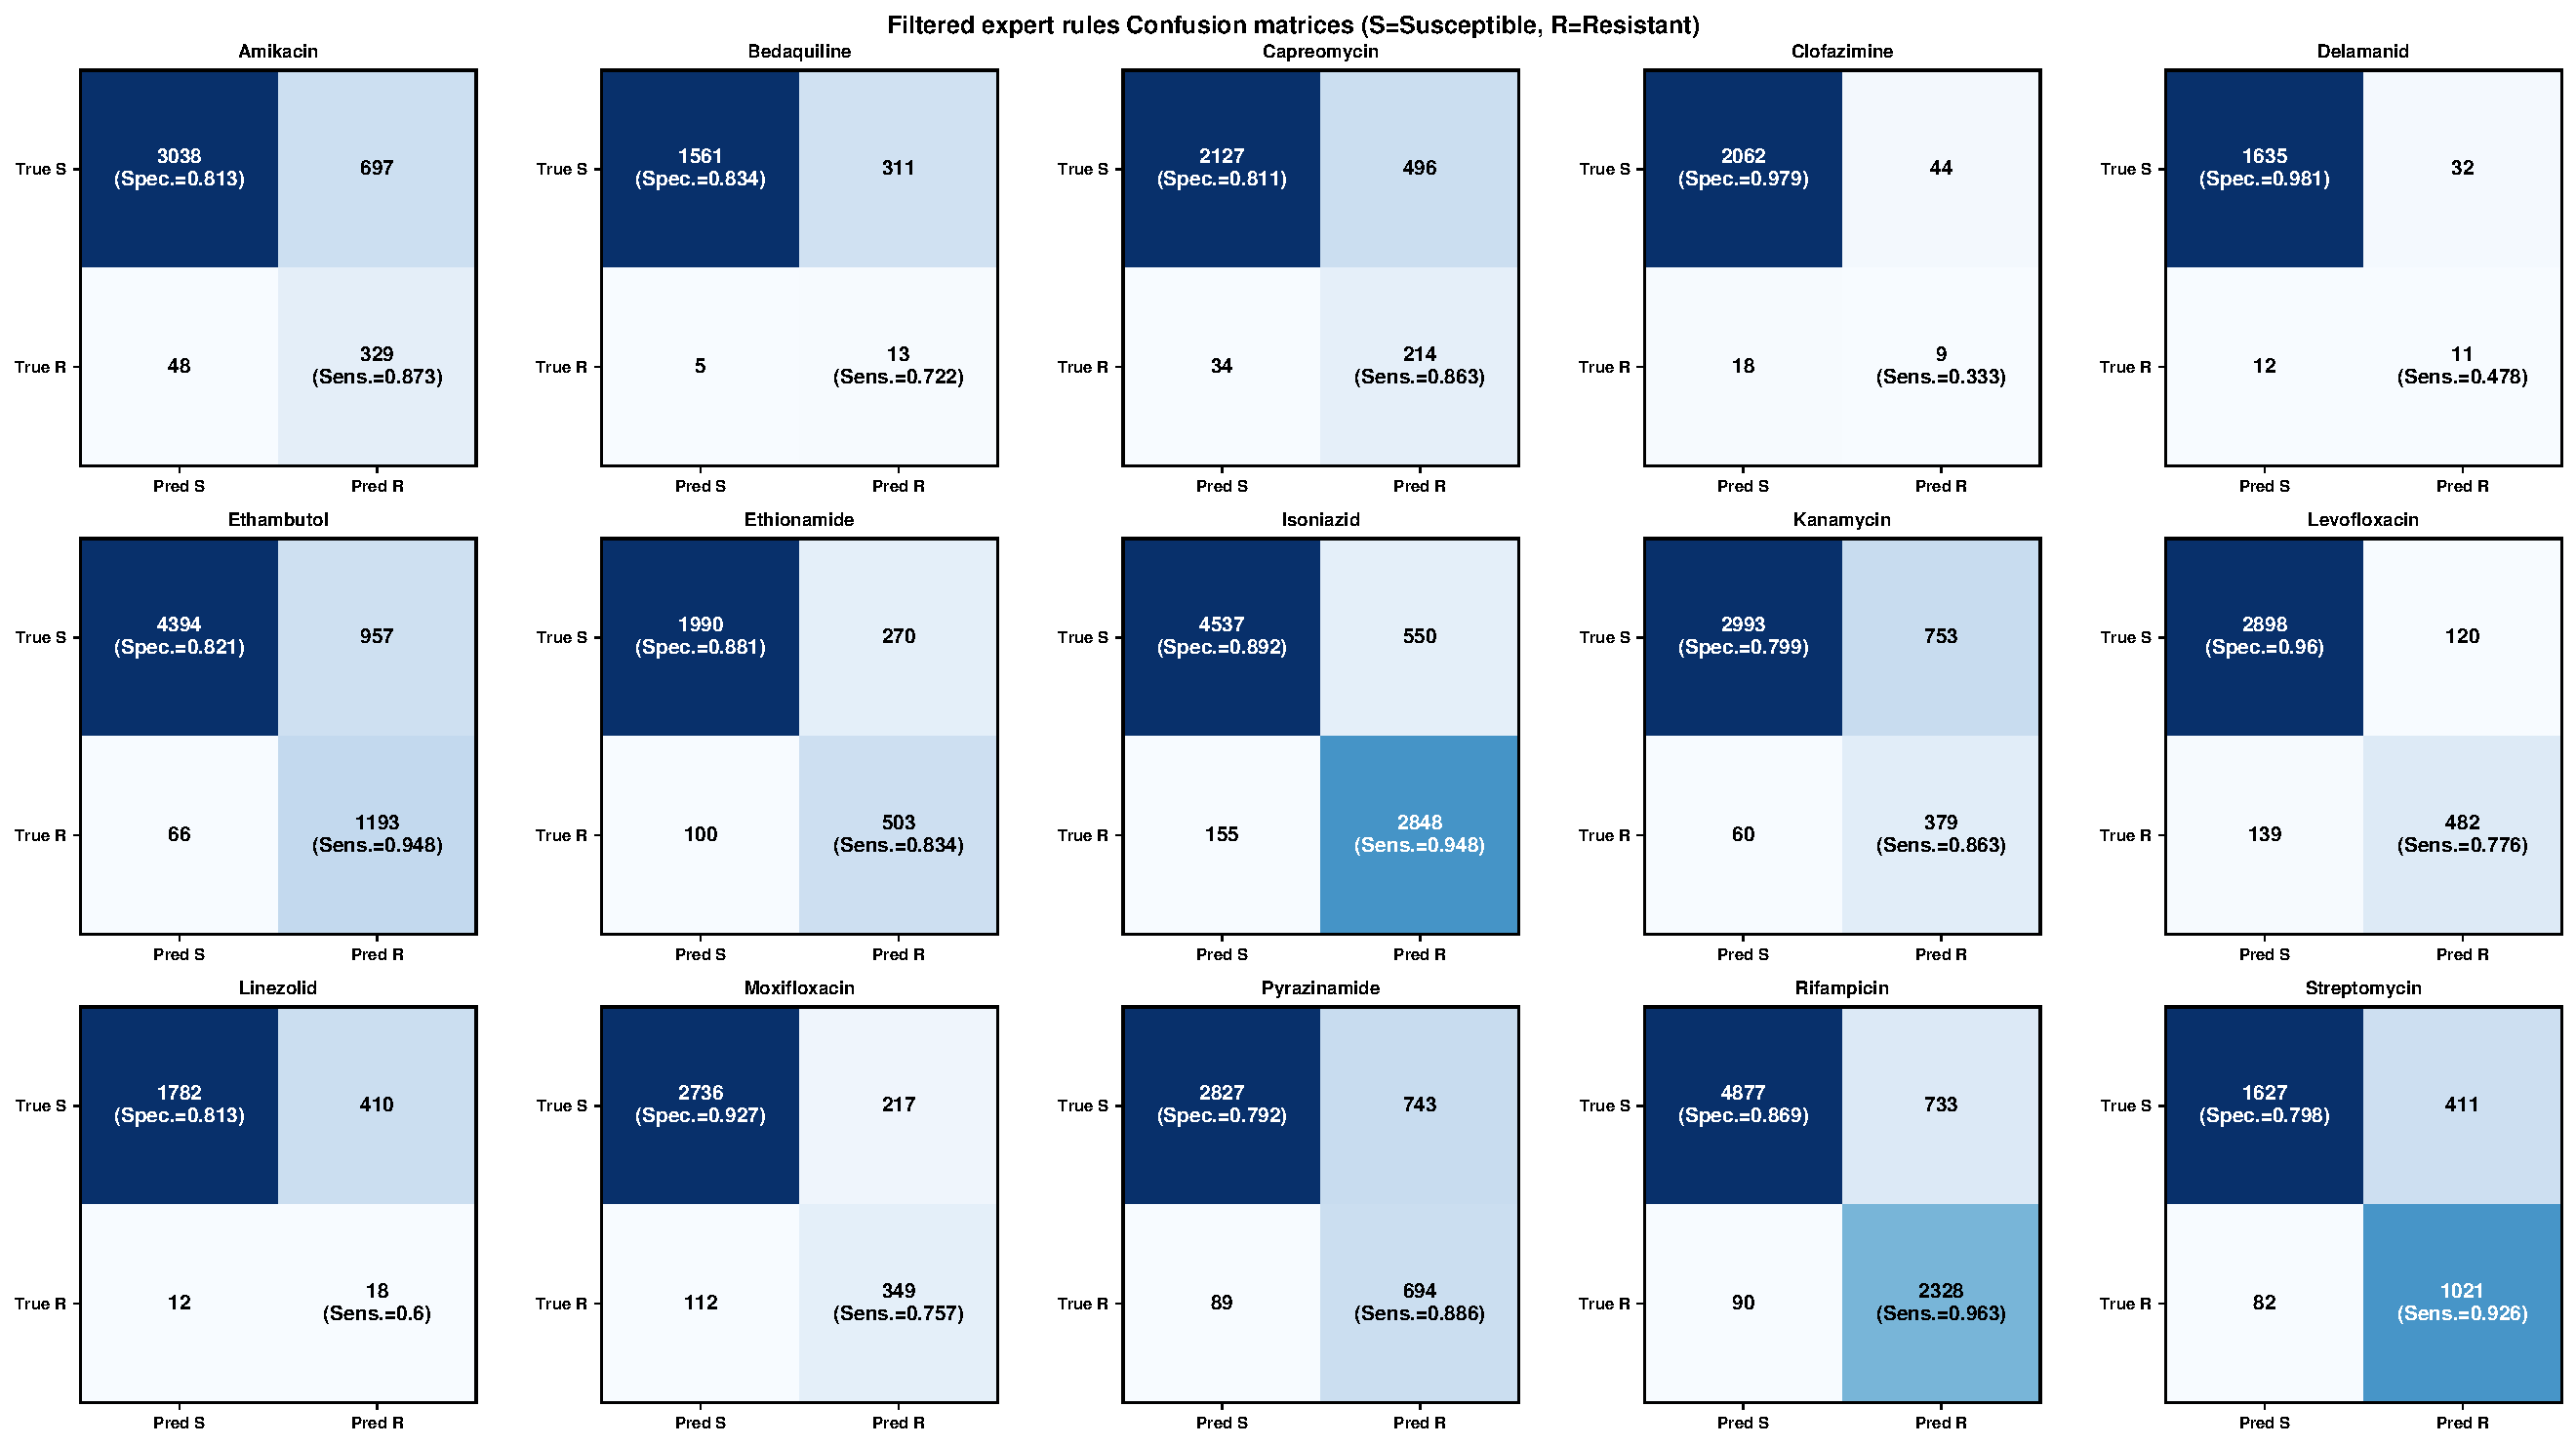
\includegraphics[width=\textwidth]{figures/filtered_expert_rules_confusion_matrices.pdf}
  \end{center}
  \caption{Confusion matrix for er+who+filt catalogue.}\label{fig:filtcm}
\end{figure}
\begin{figure}[H]
  \begin{center}
    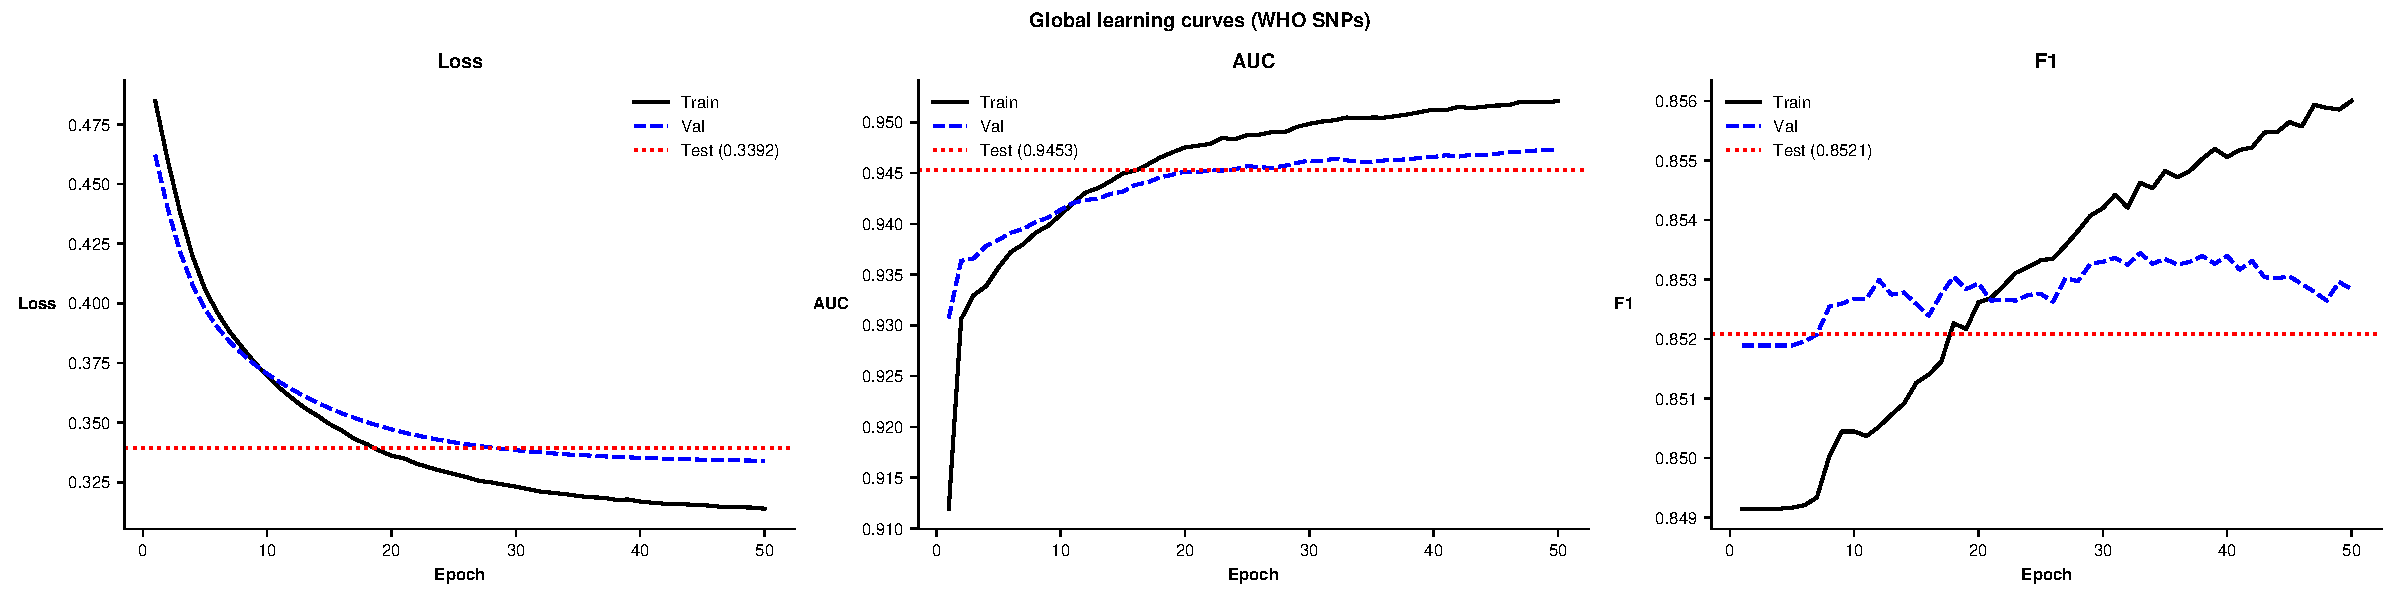
\includegraphics[width=\textwidth]{figures/who_learning_curves.pdf}
  \end{center}
  \caption{Global learning curves for who catalogue.}\label{fig:wholr}
\end{figure}

\begin{figure}[H]
  \begin{center}
    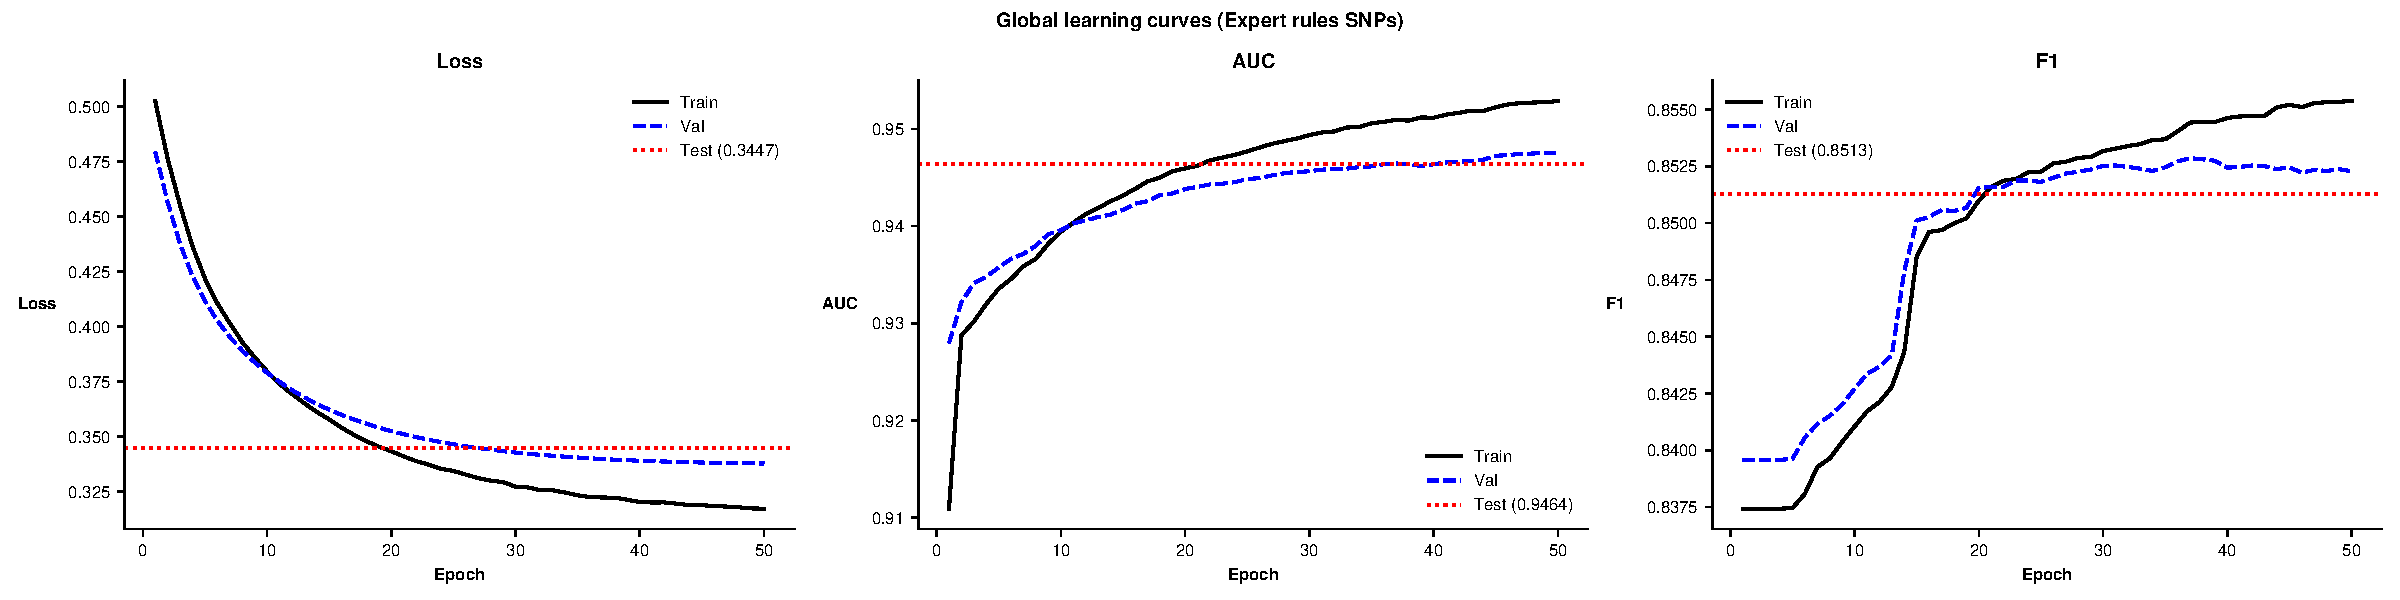
\includegraphics[width=\textwidth]{figures/expert_rules_learning_curves.pdf}
  \end{center}
  \caption{Global learning curves for er+who catalogue.}\label{fig:erlr}
\end{figure}


\begin{figure}[H]
    \centering
    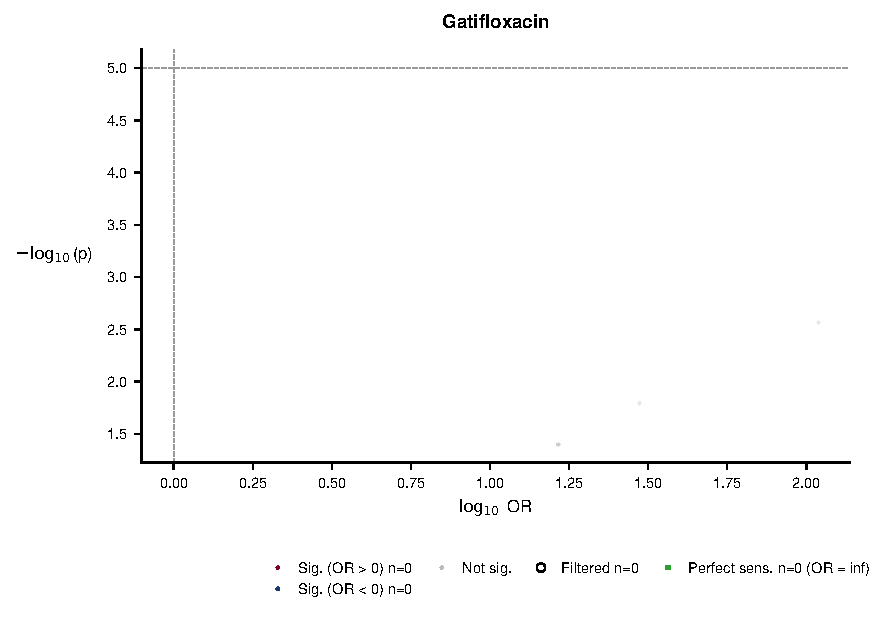
\includegraphics[width=0.45\textwidth]{./figures/plots/gatifloxacin_volcano.pdf}
    \hfill
    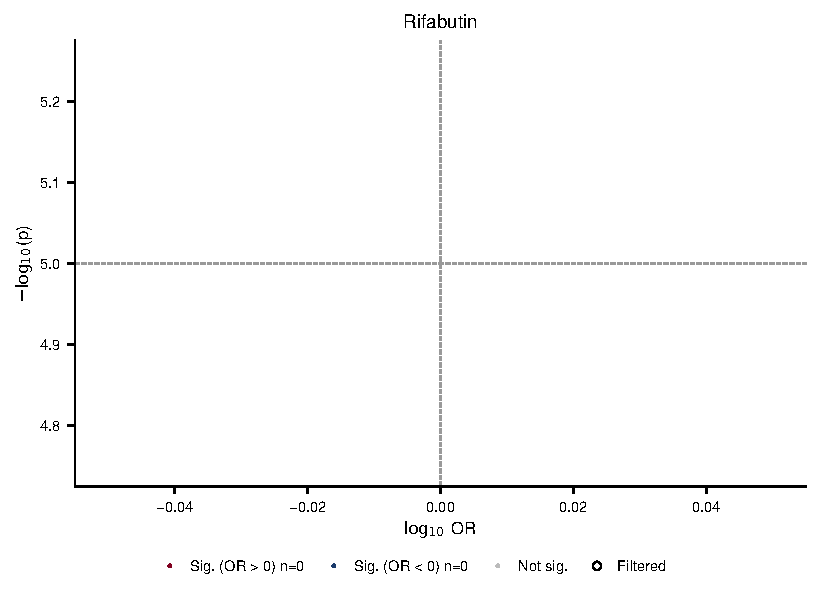
\includegraphics[width=0.45\textwidth]{./figures/plots/rifabutin_volcano.pdf}
    \hfill
\end{figure}

\end{document}
